%-----------------------------------------------------------------------------%
\chapter{\babEmpat}
%-----------------------------------------------------------------------------%
%-----------------------------------------------------------------------------%
\section{Hasil Survei dan Demografi Responden}
%-----------------------------------------------------------------------------%
Terdapat 128 tanggapan dalam survei demografi dan minat mahasiswa fasilkom pada mata kuliah Dasar Dasar Pemrograman. Hasil dari demografi responden dan analisis kuesoner akan dibahas pada bagian berikut.
\linebreak\linebreak
	Responden pada kuesoner ini terdiri dari beberapa angkatan. Angkatan yang dimaksud adalah tahun masuk responden kuliah. Terdapat 42 orang angkatan 2017 (32,6\%), 33 orang angkatan 2016 (25,6\%), 8 orang angkatan 2015 (6,2\%), 12 orang angkatan 2014 (9,3\%), dan 34 orang angkatan 2013 atau lebih lama lagi. Informasi ini dapat dilihat pada Gambar 4.1
	\begin{figure}
		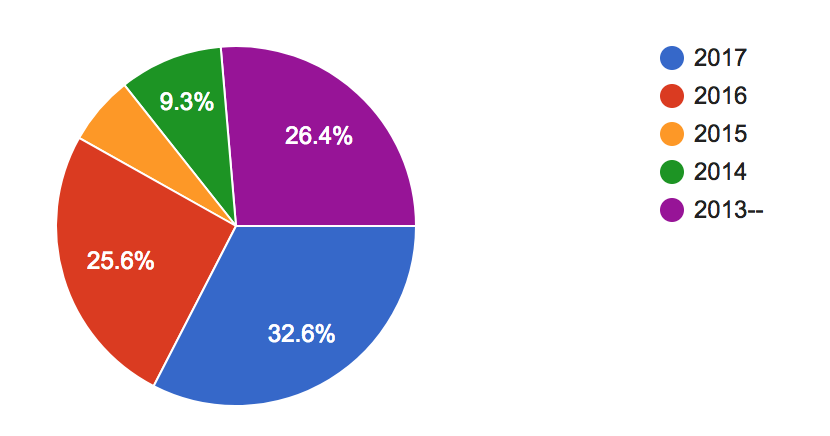
\includegraphics{pics/angkatan}
		\caption{Responden berdasarkan angkatan}
		\centering
	\end{figure}
	Responden kuesoner ini memiliki persebaran pernah mempelajari pemrograman sebelum mengikuti mata kuliah Dasar Dasar Pemograman. Responden yang pernah mempelajari pemrograman sebelum mengikuti kuliah Dasar Dasar Pemograman sebanyak 62 responden (48,8\%) dan yang belum pernah mempelajari pemrograman sebelum mengikuti kuliah Dasar Dasar Pemograman sebanyak 66 (51,2\%). Informasi ini terangkum dalam Gambar 4.2 berikut.
	\begin{figure}
		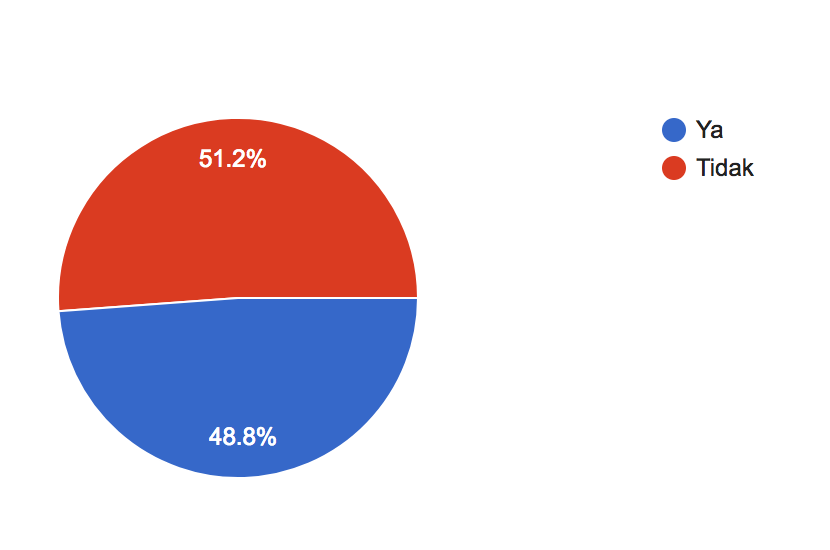
\includegraphics[width=\linewidth]{pics/pernah-ikut-ddp-sebelum}
		\caption{Responden pernah mempelajari DDP sebelumnya}
		\centering
	\end{figure}
	Dari yang telah mempelajari sebelumnya, sebanyak 42 responden mempelajarinya saat SMA, 15 responden saat SMP, dan 2 responden mempelajarinya antara SMA dan kuliah. Informasi ini terangkum dalam Gambar 4.3 berikut.
	\begin{figure}
		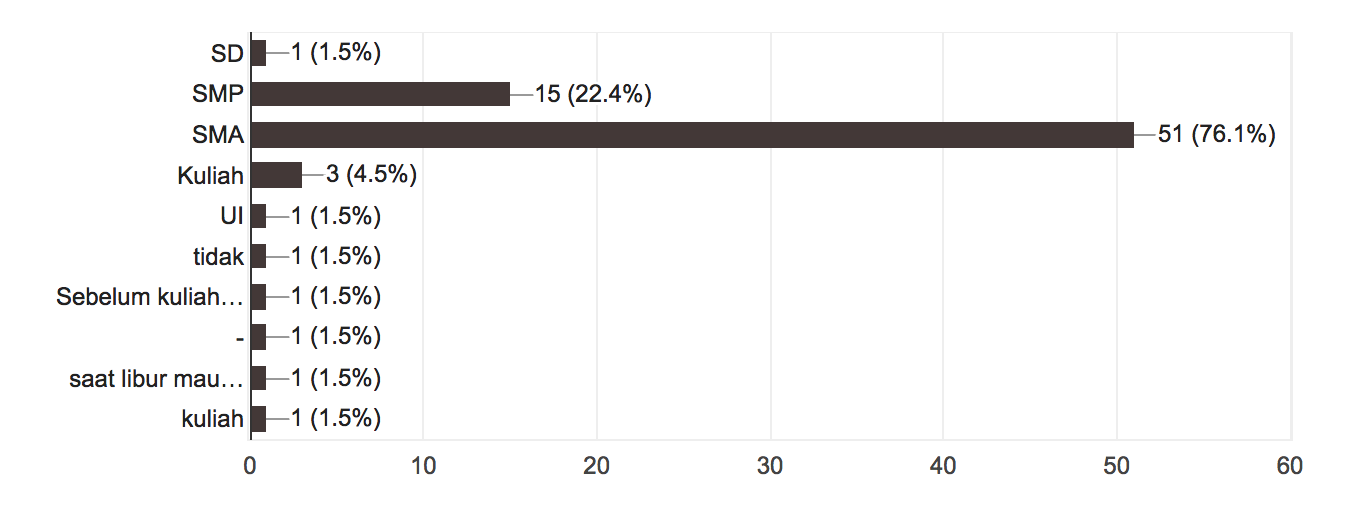
\includegraphics[width=\linewidth]{pics/kapan-pernah-belajarnya}
		\caption{Waktu mempelajari DDP}
		\centering
	\end{figure}
	Responden yang menganggap pemrograman merupakan minat mereka sebanyak 42 responden, yang mengatakan pemrograman bukan merupakan minat mereka sebanyak 14 responden, dan sebanyak 72 responden ragu untuk mengatakan pemrograman merupakan minat mereka. Informasi ini dapat dilihat pada Gambar 4.4 berikut.
	\begin{figure}
		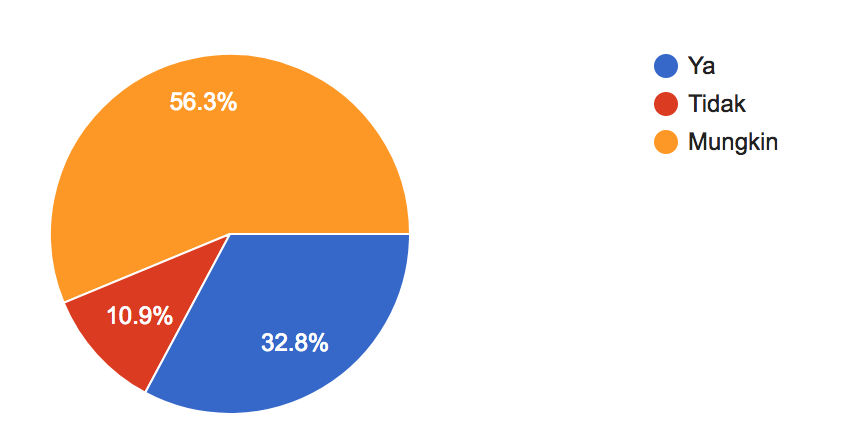
\includegraphics[width=\linewidth]{pics/passion-pemograman}
		\caption{Persebaran minat responden terhadap pemrograman}
		\centering
	\end{figure}
	Responden mengalokasikan waktu selama 3 - 5 jam dalam satu pekan untuk belajar pemrograman sebanyak 43 orang (33.6\%), 5 - 7 jam dalam satu pekan sebanyak 40 orang (31,3\%),  7 - 10 jam dalam satu pekan sebanyak 20 orang (15,6\%), kurang dari 3 jam dalam satu pekan sebanyak 17 orang (13,3\%), dan lebih dari 10 jam dalam satu pekan sebanyak 8 orang (6,3\%). Informasi ini terangkum dalam Gambar 4.5.
	\begin{figure}
		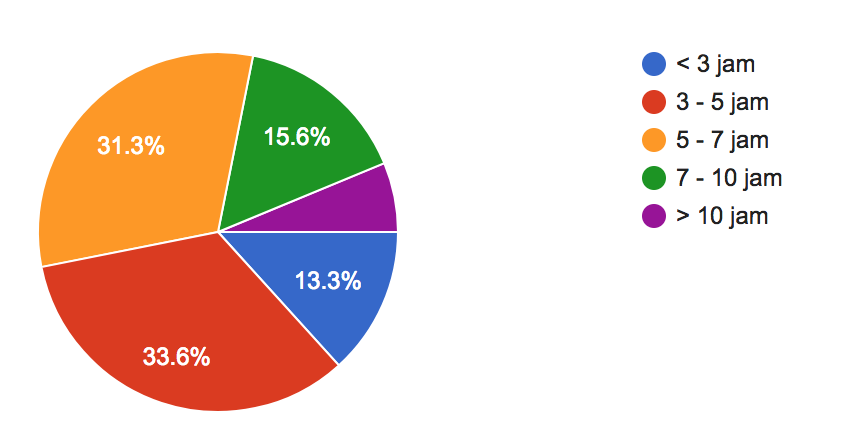
\includegraphics[width=\linewidth]{pics/lama-belajar}
		\caption{Lama belajar responden dalam satu pekan}
		\centering
	\end{figure}
	Responden diminta untuk memberikan nilai kepada dirinya sendiri sejauh mana mereka memahami pemrograman itu dengan nilai 1 - 10. Sebanyak 43 orang memberikan nilai 7, 26 orang memberikan nilai 8, 24 orang memberikan nilai 6, 11 orang memberikan nilai 5, 7 orang memberikan nilai 10, 6 orang memberikan nilai 4, 5 orang memberikan nilai 3, 4 orang memberikan nilai 2, dan 1 orang memberikan nilai 9 dan 1. Informasi ini dapat dilihat pada Gambar 4.6.
	\begin{figure}
		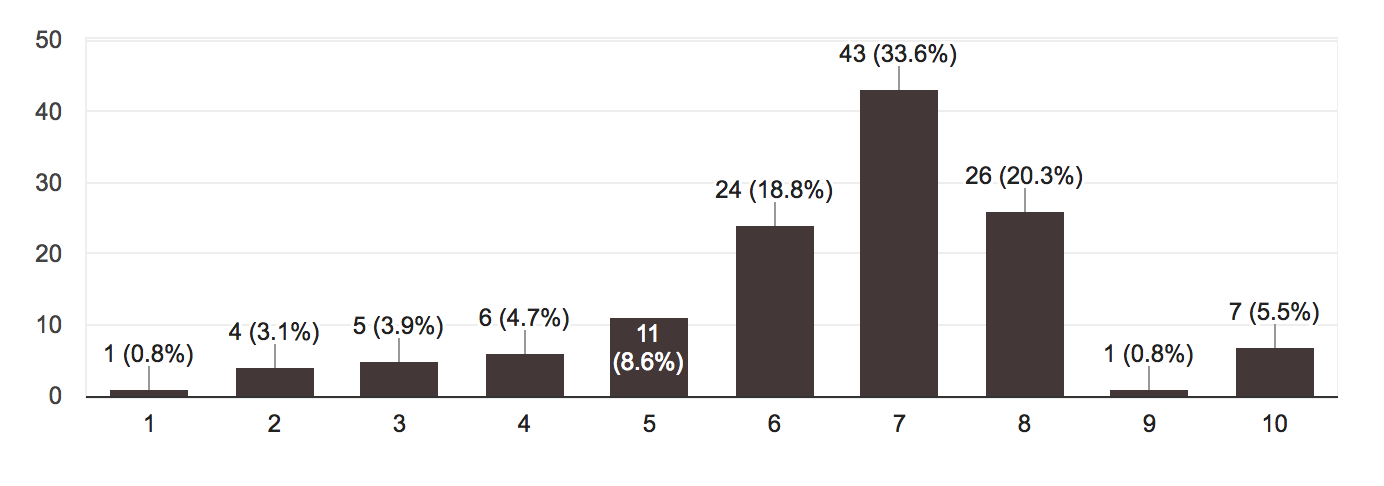
\includegraphics[width=\linewidth]{pics/nilai-pemograman}
		\caption{Nilai responden terhadap dirinya sendiri mengenai pemrograman}
		\centering
	\end{figure}
	Responden yang masuk dalam kategori sudah pernah mengambil DDP sebelumnya, terdapat 10 responden (9,6\%) yang mengulang mata kuliah DDP. dan 94 responden (90,4\%) yang tidak mengulang mata kuliah DDP. Informasi ini terdapat dalam Gambar 4.7 berikut.
	\begin{figure}
		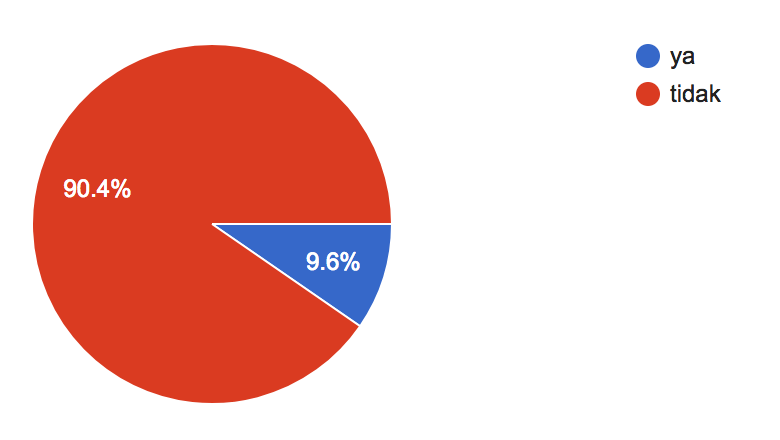
\includegraphics[width=\linewidth]{pics/mengulang-ddp}
		\caption{Persebaran responden yang mengulang}
		\centering
	\end{figure}
	Sebanyak 101 responden (78,9\%) mengatakan bahwa mereka sangat suka diberikan contoh langsung dari materi yang sedang diajarkan, 24 responden (18,8\%) suka diberikan contoh langsung, dan 3 (2,3\%) biasa saja dijika diberikan contoh langsung. informasi ini terlihat dalam Gambar 4.8.
	\begin{figure}
		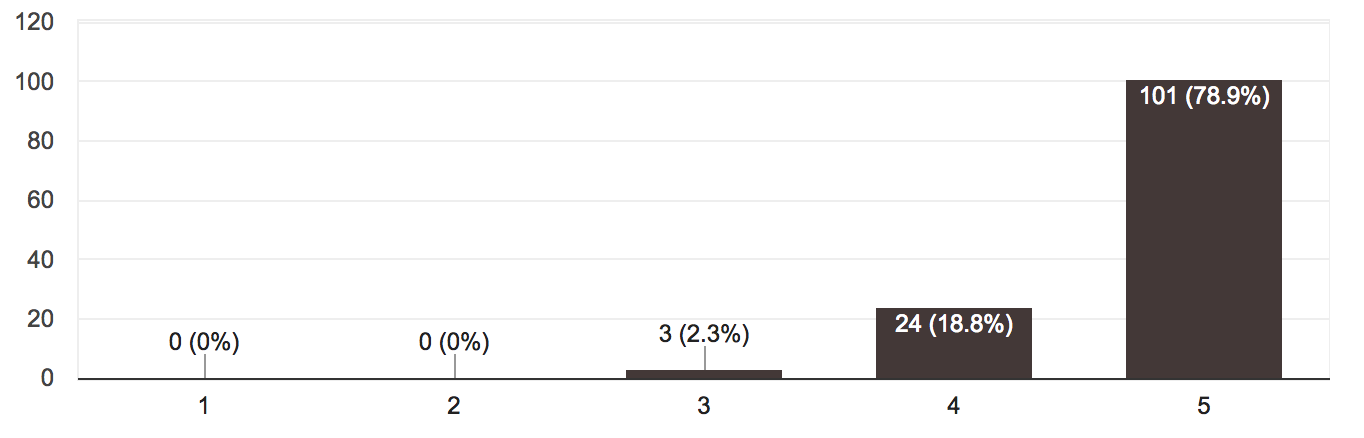
\includegraphics[width=\linewidth]{pics/contoh-langsung}
		\caption{Tingkat setuju terhadap pernyataan suka nya responden diberikan contoh langsung saat diberikan materi DDP}
		\centering
	\end{figure}
	Diberikan pernyataan bahwa responden memerlukan waktu diluar kelas untuk mempelajari lagi materi DDP. 50 responden sangat setuju, 43 setuju, 25 biasa saja, 7 tidak setuju, 3 sangat tidak setuju. Infromasi ini terkandung dalam Gambar 4.9.
	\begin{figure}
		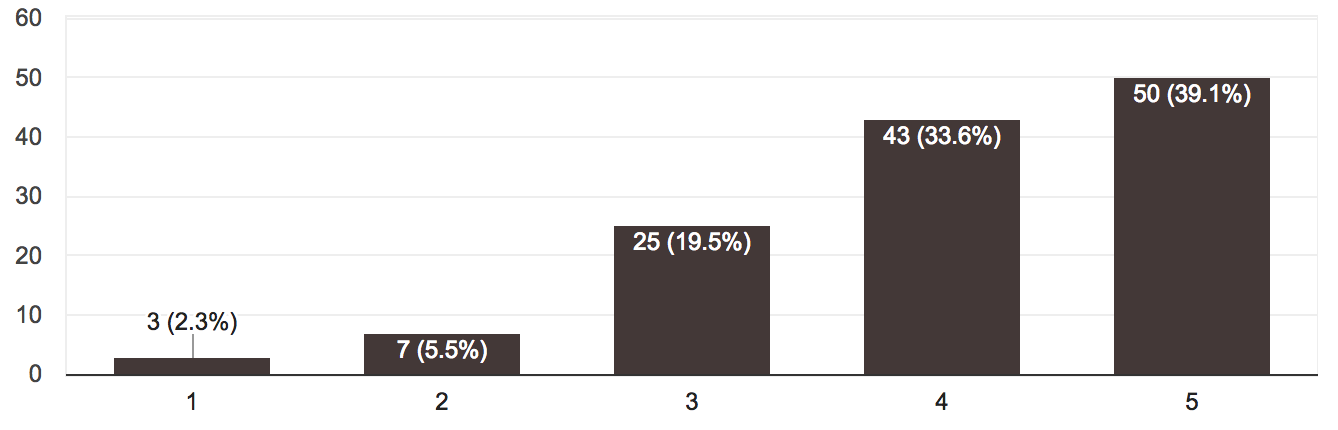
\includegraphics[width=\linewidth]{pics/perlu-waktu-luar-kelas}
		\caption{Tingkat setuju terhadap pernyataan memerlukan waktu diluar kelas untuk memahami materi DDP}
		\centering
	\end{figure}
	Sebanyak 100 responden (78,1\%)suka bermain \textit{game}, dan 28 responden (21,9\%) tidak suka bermain \textit{game}. Informasi ini terdapat pada Gambar 4.10 berikut.
	\begin{figure}
		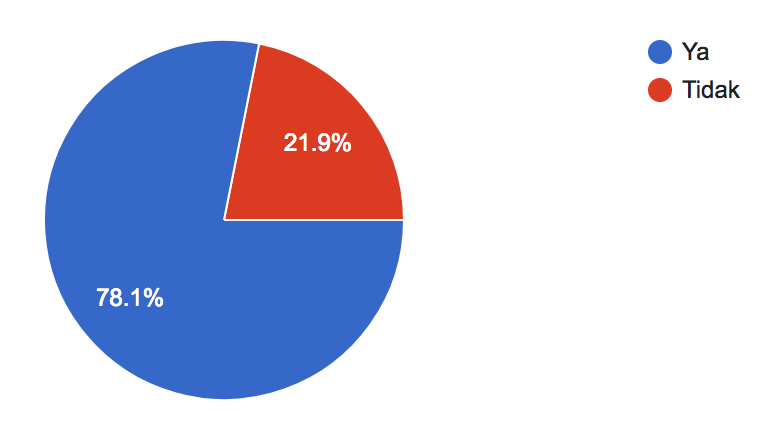
\includegraphics[width=\linewidth]{pics/suka-bermain-game}
		\caption{Menyukai bermain \textit{game}}
		\centering
	\end{figure}
	Waktu yang dihabiskan oleh 54 responden (42,2\%) kurang dari 3 jam dalam satu sepekan, 29 responden (22,7\%) 3 - 5 jam dalam satu pekan, 20 responden (15,6\%) 5 - 7 jam dalam satu pekan, 17 responden (13,3\%) lebih dari 10 jam dalam satu pekan, 8 responden (6,3\%) 7 - 10 jam dalam satu pekan. Data ini tergambarkan dalam Gambar 4.11 berikut.
	\begin{figure}
		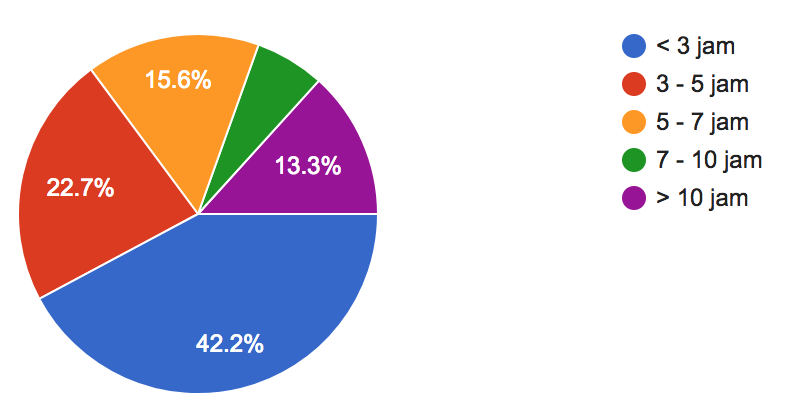
\includegraphics[width=\linewidth]{pics/waktu-bermain-game}
		\caption{Waktu yang dihabiskan bermain video permainan}
		\centering
	\end{figure}
	Responden yang lebih suka bermain \textit{game} jika dibandingkan dengan mempelajari pemrograman sebanyak 67 responden (52,3\%), 48 responden (37,5\%) ragu - ragu atau sama saja, dan 13 responden (10,2\%) mengatakan lebih suka mempelajari pemrograman dari bermain \textit{game}. Informasi ini terdapat pada Gambar 4.12 berikut.
	\begin{figure}
		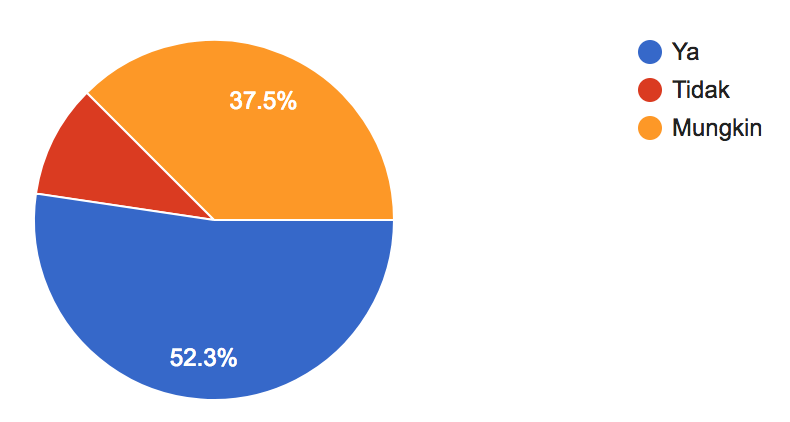
\includegraphics[width=\linewidth]{pics/lebih-senang-bermain-game}
		\caption{Persebaran lebih senang bermain \textit{game} dari belajar pemrograman}
		\centering
	\end{figure}
%
%	\begin{figure}
%		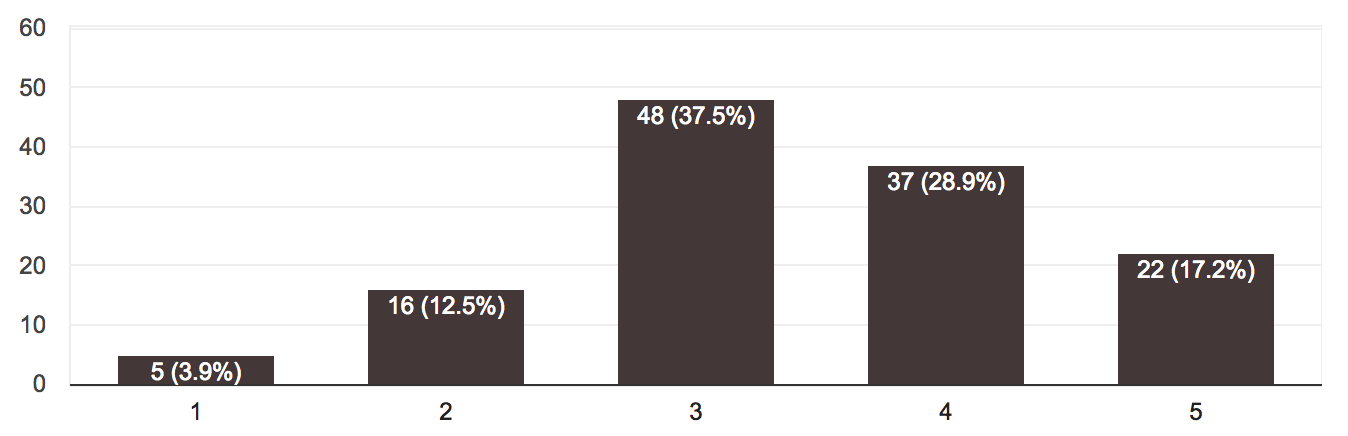
\includegraphics[width=\linewidth]{pics/menggali-lebih-dalam-sendiri}
%		\caption{Alur tahapan penelitian}
%		\centering
%	\end{figure}
%	\begin{figure}
%		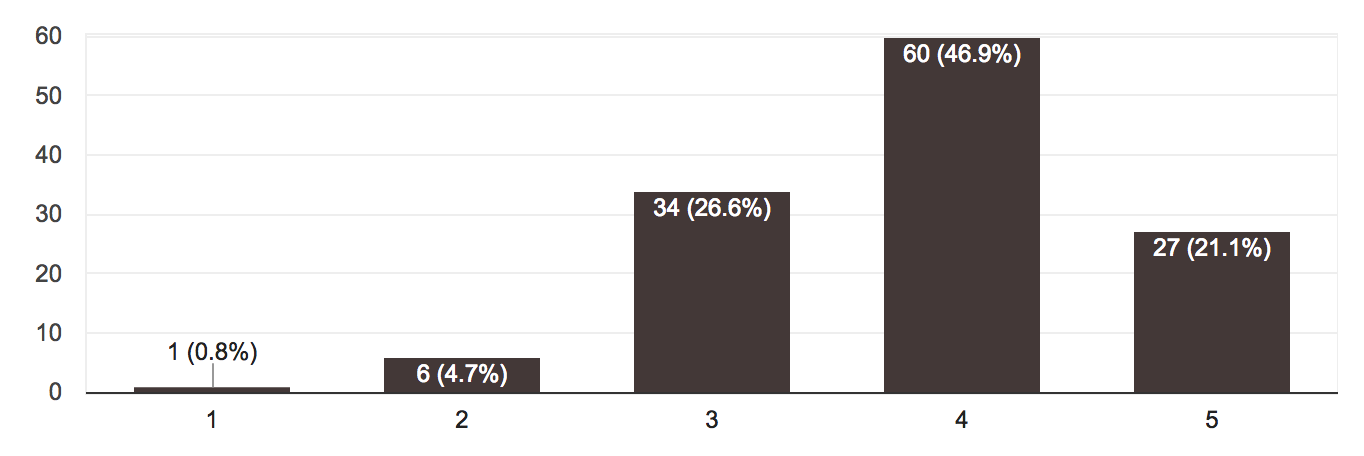
\includegraphics[width=\linewidth]{pics/menikmati-cara-belajar-sekarang}
%		\caption{Alur tahapan penelitian}
%		\centering
%	\end{figure}
%	\begin{figure}
%		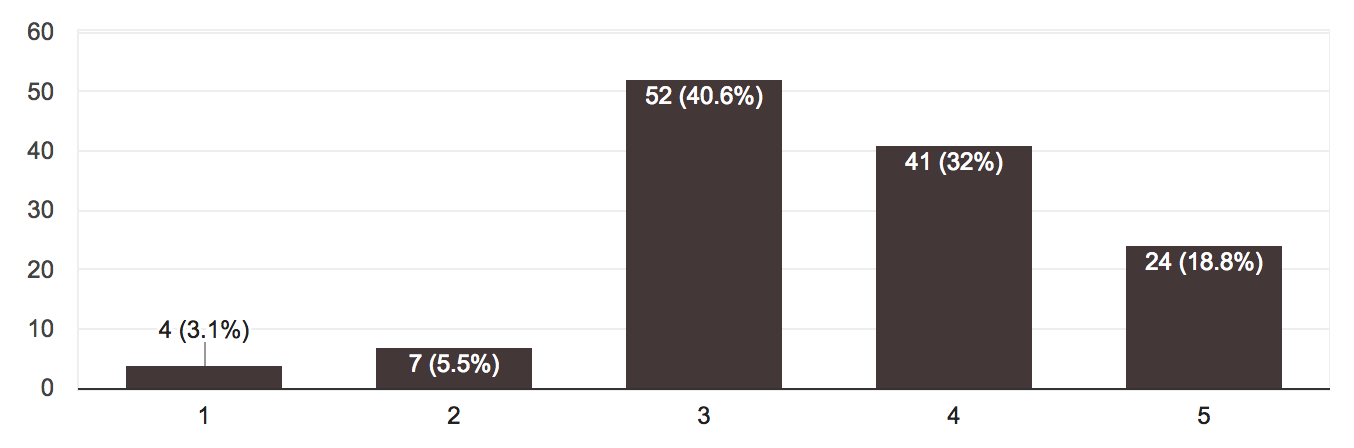
\includegraphics[width=\linewidth]{pics/mudah-memahami}
%		\caption{Alur tahapan penelitian}
%		\centering
%	\end{figure}
%	\begin{figure}
%		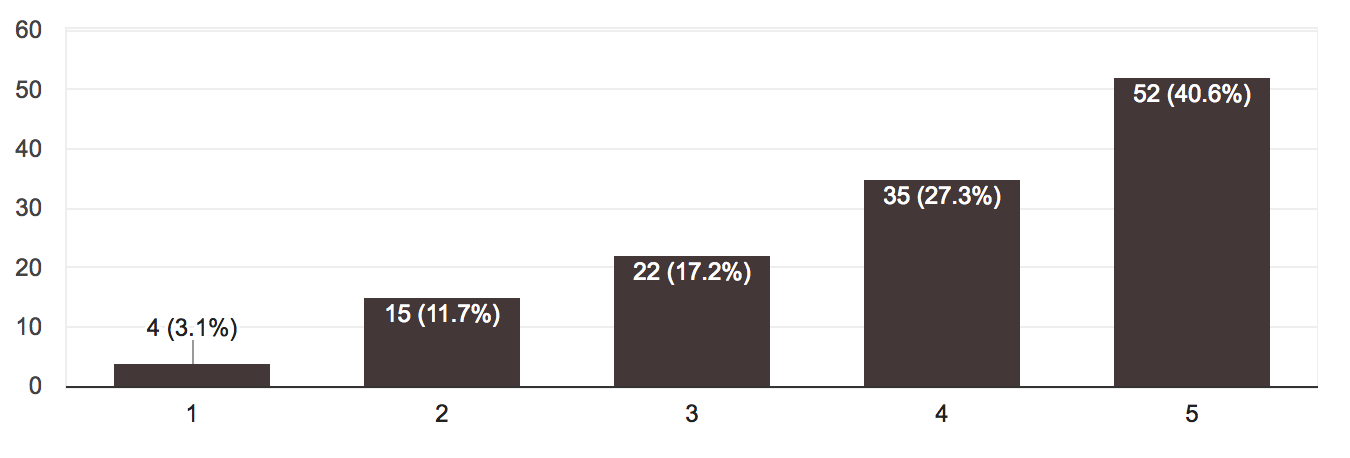
\includegraphics[width=\linewidth]{pics/slide-show-x-buku}
%		\caption{Alur tahapan penelitian}
%		\centering
%	\end{figure}
%	\begin{figure}
%		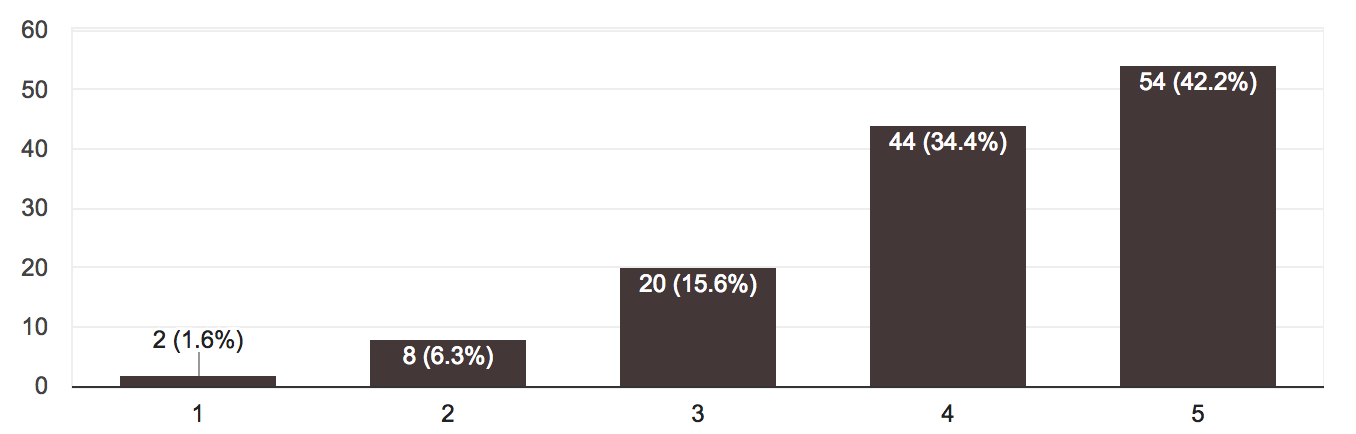
\includegraphics[width=\linewidth]{pics/tidak-suka-teori-saja}
%		\caption{Alur tahapan penelitian}
%		\centering
%	\end{figure}
% this should data kualitatif
Pada bagian \textit{open-ended} pada kuesoner, dikelompokan sesuai dengan yang telah dijelaskan pada Bab 3.2.3.
\begin{table}
	\centering
	\caption{Jenis \textit{game} yang dapat membantu pemahanan dalam belajar pemrograman}
	\label{tab:tab1}
	\begin{tabular}{| c | c | c |}
		\hline
		Kode & Konten & n \\
		\hline
		JG1 & \multicolumn{1}{p{10cm}|}{\textit{Puzzle Game}} & 53 \\ \hline
		JG2 & \multicolumn{1}{p{10cm}|}{\textit{Simulation Game}} & 28 \\ \hline
		JG3 & \multicolumn{1}{p{10cm}|}{Tidak dapat menjelaskan jenis \textit{game}} & 26 \\
		\hline
		JG4 & \multicolumn{1}{p{10cm}|}{\textit{Role-Playing Game}} & 7 \\ \hline
		PP5 & \multicolumn{1}{p{10cm}|}{\textit{Arcade Game}} & 7 \\ \hline
		JG6 & \multicolumn{1}{p{10cm}|}{\textit{Strategic Game}} & 2 \\ \hline
		JG7 & \multicolumn{1}{p{10cm}|}{\textit{Firt-Person Shooter Game}} & 2 \\ \hline
		JG8 & \multicolumn{1}{p{10cm}|}{\textit{Multiplayer Online Battle Arena}} & 2 \\ \hline
		JG9 & \multicolumn{1}{p{10cm}|}{\textit{Fighting Game}} & 1 \\ \hline
	\end{tabular}
\end{table}

\begin{table}
	\centering
	\caption{Pengertian pemrograman}
	\label{tab:tab1}
	\begin{tabular}{| c | c | c |}
		\hline
		Kode & Konten & n \\
		\hline
		PP1 & \multicolumn{1}{p{10cm}|}{membuat program} & 37 \\ \hline
		PP2 & \multicolumn{1}{p{10cm}|}{Proses dimana manusia membahasakan suatu kumpulan instruksi agar dapat dimengerti dan dijalankan oleh komputer} & 34 \\ \hline
		PP3 & \multicolumn{1}{p{10cm}|}{\textit{Problem solving} atau penyelesaian sebuah masalah} & 27 \\
		\hline
		PP4 & \multicolumn{1}{p{10cm}|}{Tidak dapat mengartikan pemrograman} & 15 \\ \hline
		PP5 & \multicolumn{1}{p{10cm}|}{Serangkaian kode untuk mencapai tujuan tertentu} & 13 \\ \hline
		PP6 & \multicolumn{1}{p{10cm}|}{Pola pikir} & 1 \\ \hline
		PP7 & \multicolumn{1}{p{10cm}|}{Mempelajari bahasa pemrograman} & 1 \\ \hline
		PP8 & \multicolumn{1}{p{10cm}|}{Jembatan komunikasi antara manusia dengan teknologi} & 1 \\ \hline
	\end{tabular}
\end{table}

\section{Relevansi Landasan Teori}
Pada subbab ini akan diberikan hasil relevansi teori dengan sistem yang akan dibuat. Relevansi ini akan ditampilkan dalam bentuk tabel.
\begin{longtable}{| p{2cm} | p{5cm} | p{5cm} |}
	%\centering
	\caption{Relevansi landasan teori} \\
	\hline
	\textbf{Landasan teori} & \textbf{Deskripsi singkat yang didapatkan} & \textbf{\textit{Requirement} yang dapat disimpulkan} \\
	\hline
	\endfirsthead
	%\begin{tabular}{| p{2cm} | p{5cm} | p{5cm} |}
		\hline
		\textbf{Landasan teori} & \textbf{Deskripsi singkat yang didapatkan} & \textbf{\textit{Requirement} yang dapat disimpulkan} \\
		\hline
		\endhead
		Teori Perancangan Game & Jenis \textit{game} berdasarkan media dimana dimainkannya adalah \textit{board game, card game, athletic game}, dan \textit{computer game}. & Penelitian ini merupakan pembelajaran berbasis komputer, sehingga jenis yang dipilih adalah \textit{computer game}. \\
		\hline
		& \textit{Game} memiliki banyak jenis seperti \textit{Action Game, Adventure Game, Fighting game, Puzzle Game, Role-Playing Game}, dan \textit{Simulation Game}. & Mendapatkan hasil kuesoner tentang jenis \textit{game} yang dapat membantu pembelajaran pemrograman adalah \textit{puzzle} dan \textit{simulation game}\\
		\hline
		Teori pembelajaran & Bloom Taxonomy merupakan yang sering digunakan dalam bidang pendidikan terutama pembelajaran berbasis komputer. & Tahap yang harus dicapai dalam pengenalan dasar dasar pemrograman adalah \textit{Application}. Pengguna harus mampu melakukan menyelesaikan permasalahan terkait dengan menggunakan konsep \textit{Computational Thinking }. \\
		\hline
		Pembelajaran berbasis permainan & Terdapat tiga puluh enam butir prinsip yang dikemukakan dalam pengembangan pembelajaran berbasis \textit{game} (JP Gee 2003). & Setiap butir akan menjadi pertimbangan dalam merancang dan menjelaskan setiap tahap pada sistem. \\
		\hline
		& Terdapat empat model pembelajaran berbasis komputer (Budianto 2014) yaitu \textit{drill}, tutorial, simulasi, dan \textit{instructional game}. & Berbasis pada metode \textit{drill}, tantangan dalam  \textit{game} ini harus mampu memberikan pelatihan berulang kepada peserta didik sehingga diharapkan materi tersebut tertanam dan menjadi kebiasaan. Berbasis pada metode \textit{instructional game}, maka harus terdapat tujuan pembelajaran yang dicapai, aturan game yang didefinisikan dalam \textit{requirement}, dan kompetisi terhadap diri sendiri untuk maju ke level selanjutnya. Tantangan yang harus mendefinisikan tujuan. \\
		\hline
		\textit{Computational Thinking} & Tiga permasalahan utama \textit{Computational Thinking} adalah permasalahan yang dihadapi, membuat desain solusi yang sistematis, dan pendekatan solusi berdasarkan perilaku manusia. & Permasalahan yang dihadapi adalah tantangan setiap tahap. Pengguna akan membuat solusi yang sistematis dari setiap tantangan yang ada. Solusi dari tantangan setiap tahap harus berbasis pada perilaku manusia dan terdapat pemanfaatan dari teori dalam ilmu komputer. \\ 
		\hline
		Desain Antarmuka & Terdapat delapan aturan emas yang menjadi pedoman dalam membuat desain interaksi. & Setiap poin akan menjadi pertimbangan dalam menentukan desain antarmuka yang akan dibuat. Seperti poin \textit{Strive For Consistency} menentukan jika telah menggunakan \textit{font} satu maka akan digunakan diberbagai tempat tempat dan jika suatu tombol memiliki perintah tertentu maka disetiap tempat akan memiliki perintah yang sama \\ 
		\hline
		Dasar Dasar Pemrograman 1 & Terdapat 15 topik yang akan diajarkan pada mata kuliah Dasar Dasar Pemrograman 1 & Dengan mempertimbangkan kemampuan dan kemudahan dalam pengembangan prototipe maka ditentukan materi konsep \textit{repetition} atau iterasi \\ \hline
	%\end{tabular}
\end{longtable}

\section{Mendefinisikan Persona dan Spesifikasi Sistem}
Pada subbab ini akan diberikan hasil dari hasil survei dan demografi yang dipaparkan pada Subbab 4.1. Setelah didapatkan hasil maka terbentuk persona yang menjadi gambaran umum dari responden dan juga spesifikasi sistem yang akan dibuat dari estetika, mekanik, teknologi dan naratifnya.

	\subsection{Persona}
	Persona ditentukan berdasarkan demografi responden terbanyak pada kuesioner adalah mahasiswa yang sudah menerima pelajaran pemrograman dari sebelum kuliah dan persona kedua adalah belum menerima pelajaran pemrograman dari sebelum kuliah. Berikut merupakan gambaran kedua persona tersebut.
	\begin{figure}
		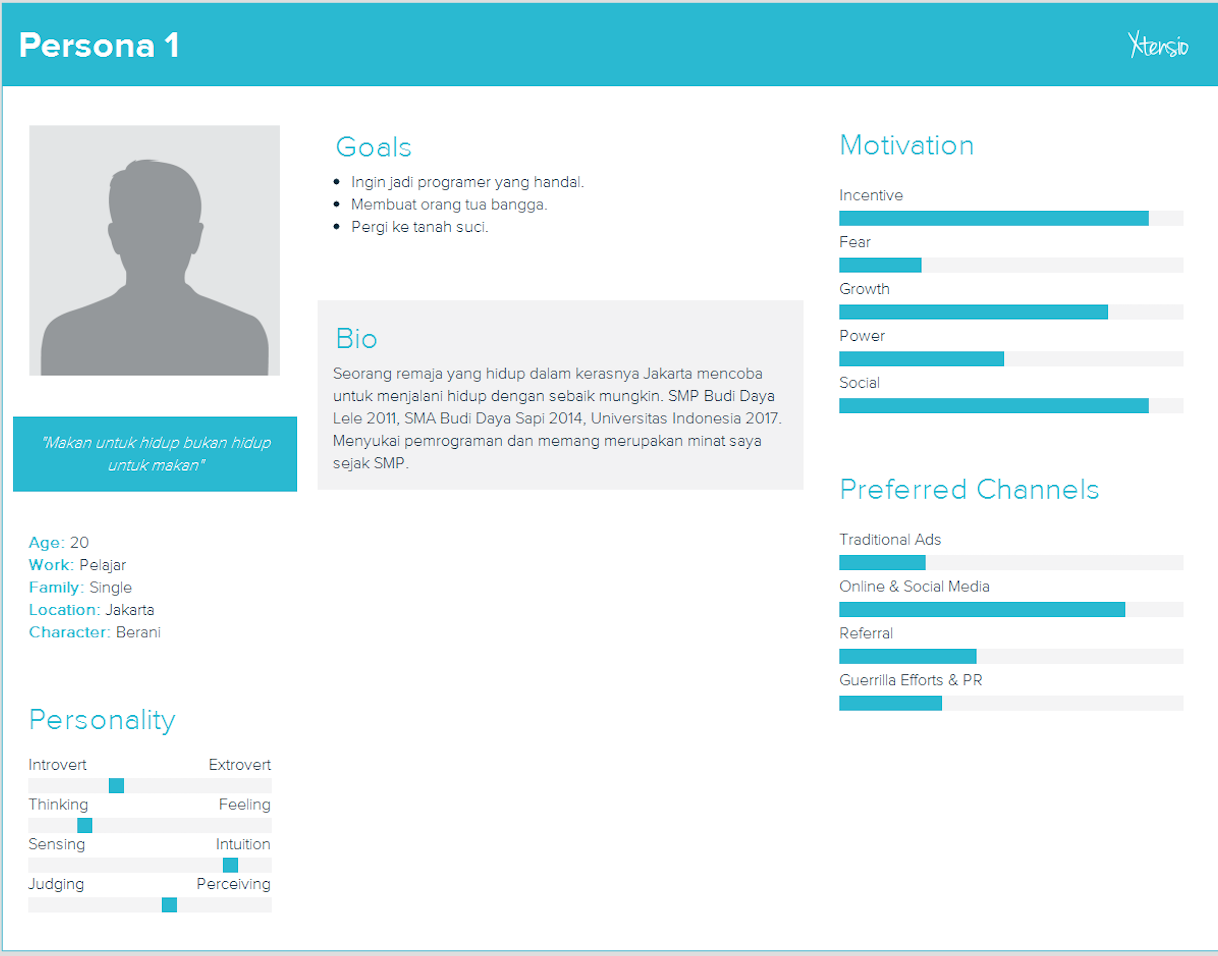
\includegraphics[width=\linewidth]{pics/pesona1}
		\caption{Persona 1}
		\centering
	\end{figure}
	\begin{figure}
		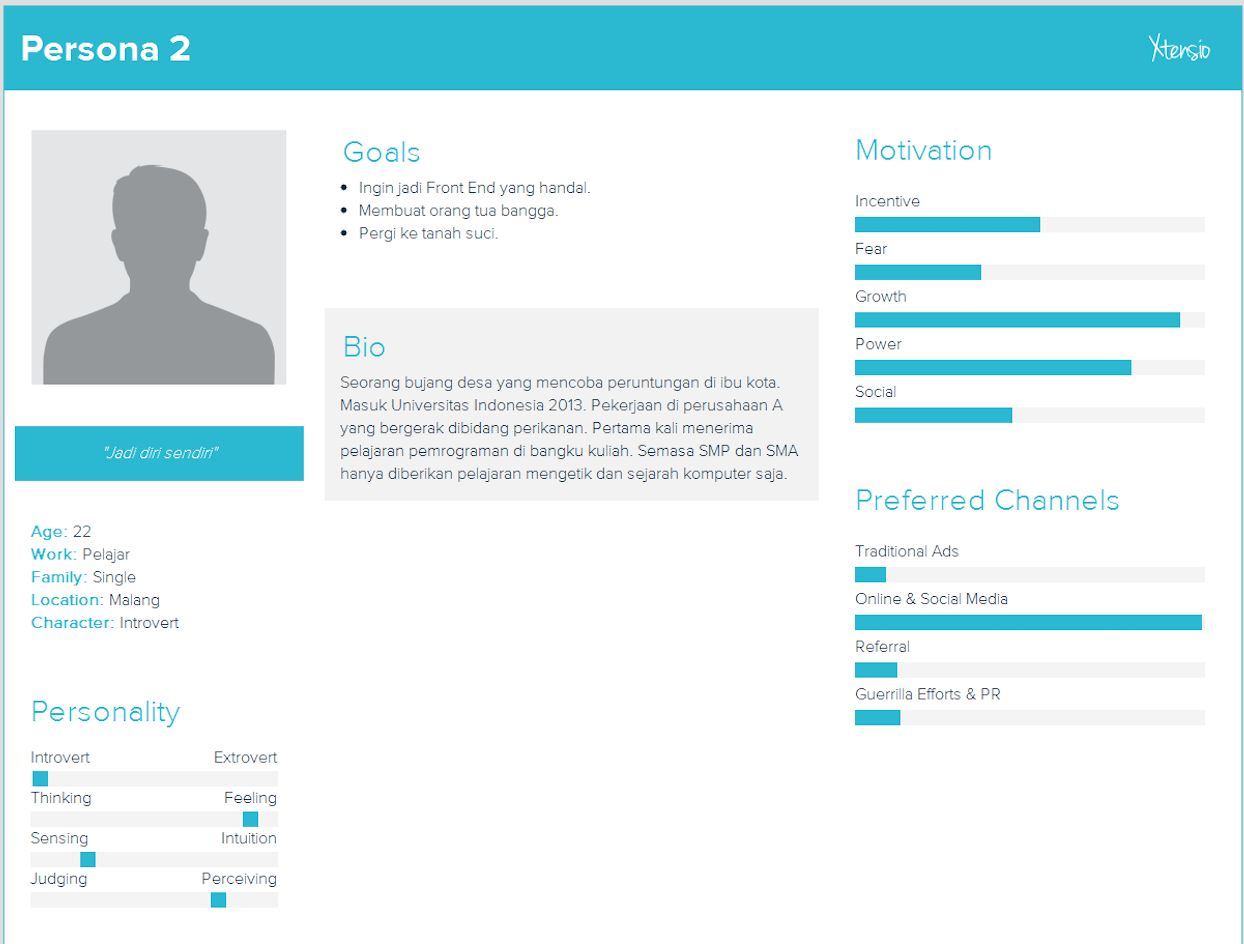
\includegraphics[width=\linewidth]{pics/pesona2}
		\caption{Persona 2}
		\centering
	\end{figure}
	\subsection{Spesifikasi Sistem}
		Spesifikasi sistem dikaitkan dengan hasil dari kuesoner \textit{online} dan hasil relevansi landasan teori. Dalam penerapan \textit{game design} terdapat empat elemen yang terkait hasil kuesoner. Keempat elemen yang dihasilkan sebagai berikut:
		\begin{itemize}
			\item Naratif
				\subitem Permainan ini berceritakan seorang pembalap yang sedang kesulitan mencari jalan keluar untuk menyelesaikan suatu tahap. Dalam setiap tahap pembalap harus mengumpulkan semua koin yang tersedia untuk menuju tahap berikutnya. Pembalap tidak boleh keluar jalur atau dia akan dikeluarkan dari balapan tersebut.
			\item Estetika
				\vadjust{\penalty10000}
				\subitem Tema yang diambil untuk sistem ini adalah retro. Aset yang digunakan diambil dari asset yang disedian gratis oleh teknologi yang dipakai. Aset yang diambil sebagai berikut:
				\begin{figure}
					\centering
					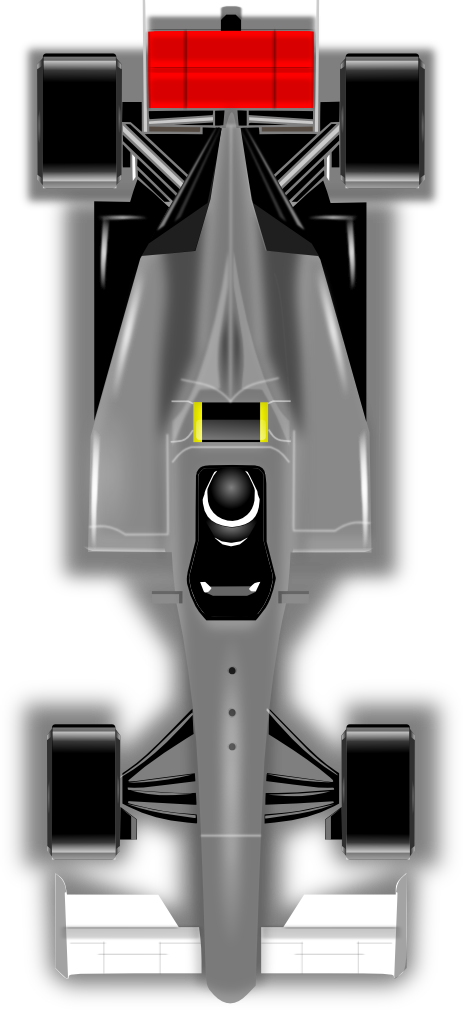
\includegraphics[width=70pt]{pics/aset/1}
					\caption{Karakter utama}
				\end{figure}
				\begin{figure}
					\centering
					
\includegraphics[width=70pt]{pics/aset/2}
					\caption{Asset jalanan}
				\end{figure}
			\item Mekanik
				\subitem Mekanik yang dikembangkan akan didasari oleh \textit{puzzle game}. Hal ini juga tergambarkan pada kuesoner kode JG yang memiliki frekuensi paling banyak, yaitu \textit{puzzle game}. Pemain akan diminta menyelesaikan sebuah masalah yang terdapat pada setiap tahap untuk mencapai tahap selanjutnya.
				\subitem Pemain akan mendapatkan poin dari setiap tahap yang diselesaikan. Pemain akan memiliki kontrol yaitu \textit{tap} dan menulis kode. Terdapat tiga buah kotak yang menjadi pokok utama permainan. Pada kotak sebelah kanan akan ditampilkan sebuah masalah yaitu sebuah mobil yang harus berjalan sesuai lintasan dan juga harus mendapatkan semua koin yang tersebar dalam lintasan tersebut. Pada kotak bagian tengah pemain dapat menuliskan kode yang harus Pemain harus menuliskan kode pada bagian \textit{input field}, lalu menjalankan dengan menekan tombol "\textit{run}". Dengan menekan tombol tersebut, maka sang pembalap akan bergerak sesuai dengen kode yang ditulis oleh pemain. Kotak paling kanan sebagai \textit{Head-Up Display} (HUD) yang menampilkan nilai, tahap, jumlah koin tersisa dan tulisan bantuan untuk mengerjakan 
			\item Teknologi
				\subitem Pada sistem digunakan \textit{game engine} Unity 2017 sebagai alat bantu utama. Pemilihan Unity 2017 karena \saya lebih terbiasa dengan Unity 2017 dari \textit{game engine} yang lainnya. Memilih \textit{game engine} yang paling terbiasa akan menyebabkan tingkat \textit{development} lebih cepat. Selain itu Unity 2017 juga memiliki banyak \textit{library} dan aset gratis. Unity 2017 juga menyediakan \textit{Integrated Development Environment} (IDE) yaitu Mono Develop.
				\subitem Kemudian Git digunakan sebagai \textit{source code management} dan \textit{version control system} serta Github sebagai \textit{repository hosting service}-nya. Penggunaan Git sangat membantu dalam pengerjaan dibeberapa gawai.
				\subitem Alat bantu lainnya adalah Google Drive yang digunakan sebagai \textit{cloud storage}. Penyimpanan awan ini digunakan untuk menyimpan versi dari prototipe yang telah selesai.
		\end{itemize}

\section{Perancangan Desain Prototipe}

	\subsection{Perancangan Menu Utama}
	Pada bagian menu utama akan dibuat tampilan menu pada umumnya, yaitu terdapat judul permainan, ikon permainan, dan juga beberapa tombol perintah. Judul permainan akan ditempatkan pada tengah atas bagian dan ikon tepat di bawah judul dari permainan ini. Tombol perintah akan berada di bawah ikon permainan, lalu terdapat tombol pengaturan dan keluar permainan yang terpisah, karena ini bukan merupakan bagian dari permainannya. Berikut pada Gambar 4.17.
	\begin{figure}
		\centering
		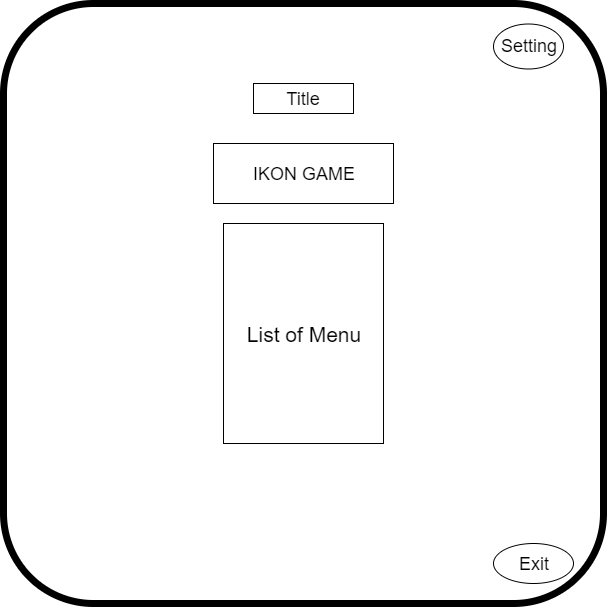
\includegraphics[width=\linewidth-80pt]{pics/low/low1}
		\caption{Tampilan \textit{Low fidelity} halaman menu utama}
	\end{figure}
	
	\subsection{Perancangan Menu Pengaturan}
	Pada menu pengaturan terdapat tombol perintah untuk mengatur aturan dasar permainan ini, seperti volume atau resolusi layar. Paling bawah dari tombol perintah tersebut adalah tombol kembali ke halaman menu utama. Pada Gambar 4.18 merupakan gambaran kasar dari menu pengaturan ini.
	\begin{figure}
		\centering
		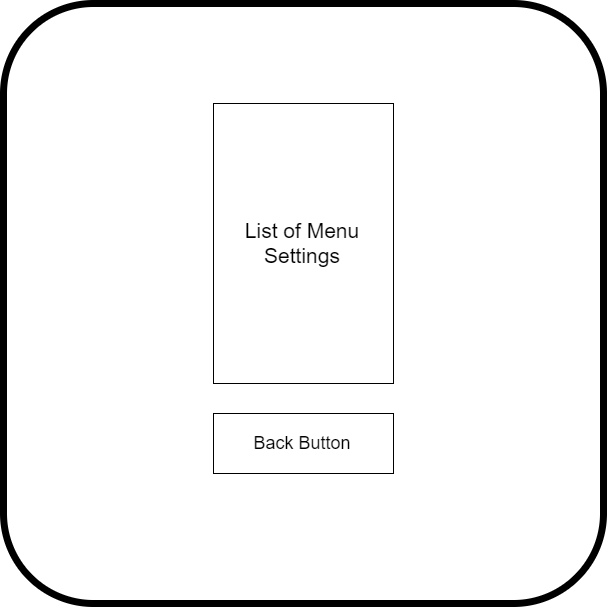
\includegraphics[width=\linewidth-140pt]{pics/low/low2}
		\caption{Tampilan \textit{Low fidelity} halaman menu pengaturan}
	\end{figure}
	
	\subsection{Perancangan Halaman Utama Bermain}
	Pada halaman utama bermain terdapat 3 komponen utama. Komponen pertama adalah konten \textit{puzzle} yang terdapat pada kiri layar. Pada komponen ini akan ditampilkan konten atau masalah apa yang akan di selesaikan oleh pengguna. Setelah itu komponen yang berada di tengah adalah \textit{text editor} untuk mensimulasikan bagaimana cara menulis kode. Komponen yang terakhir berada pada kanan yaitu HUD. Tampilan halaman bermain akan ada pada Gambar 4.19.
	\begin{figure}
		\centering
		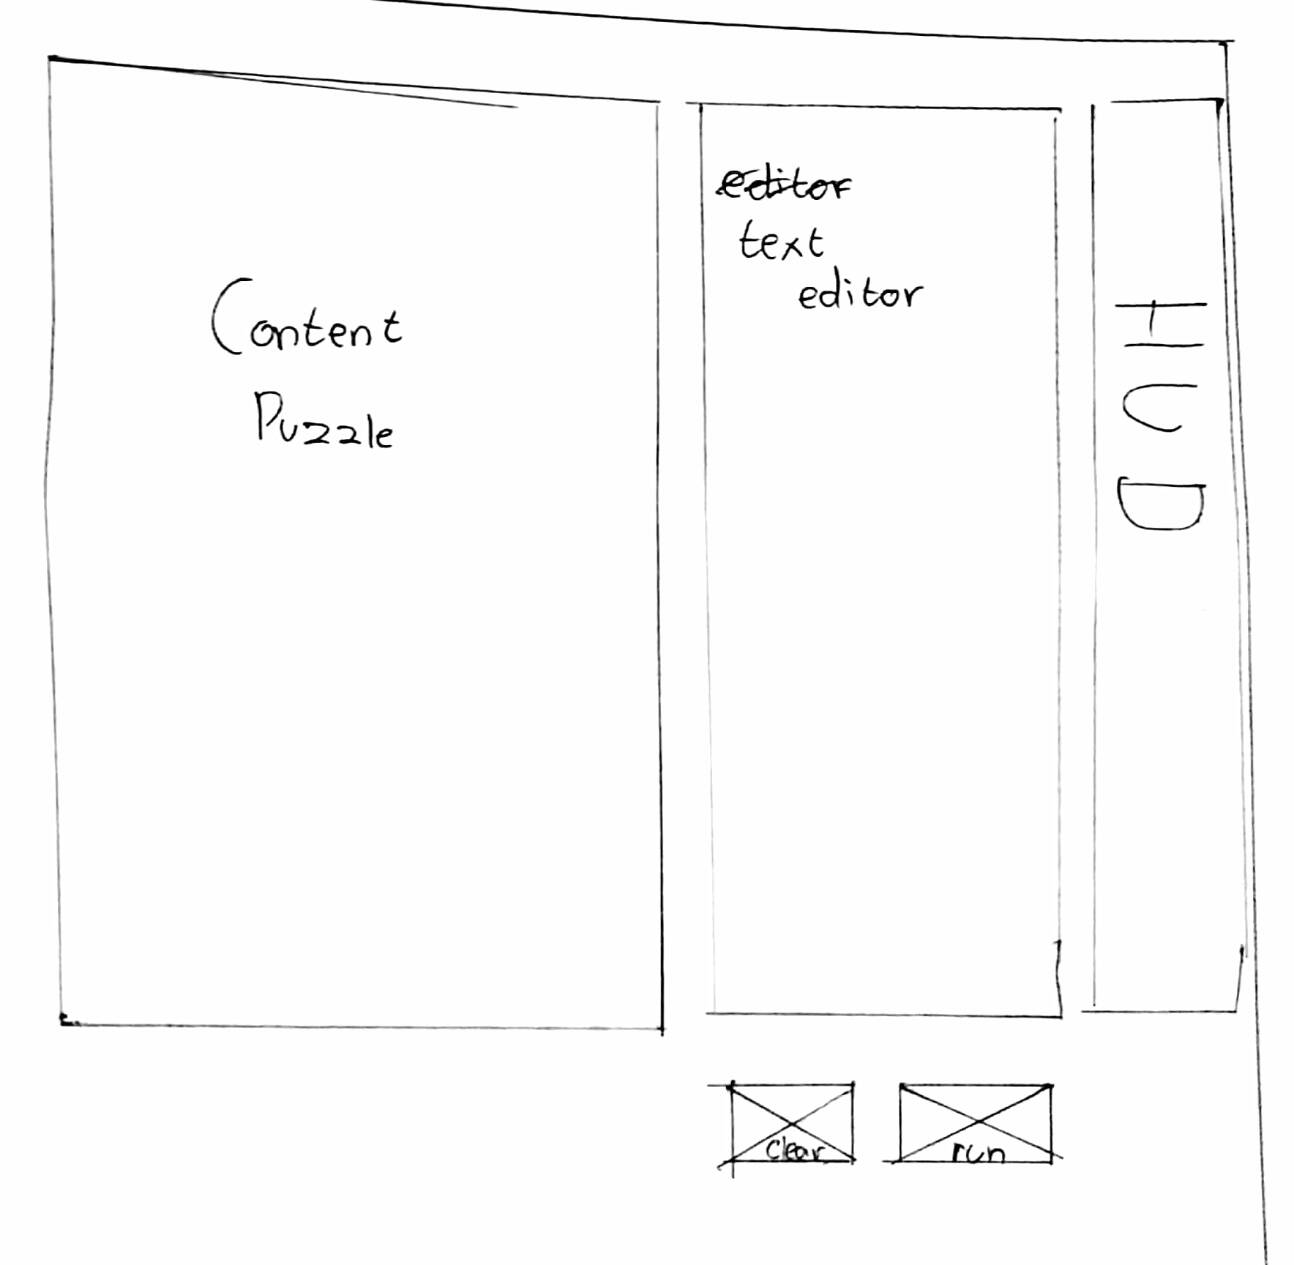
\includegraphics[width=\linewidth-80pt]{pics/low/low3}
		\caption{Tampilan \textit{Low fidelity} halaman utama untuk bermain}
	\end{figure}
	
	\subsection{Perancangan Halaman Setelah Menyelesaikan Tahap}
	Halaman ini merupakan \textit{reward} yang diberikan kepada pengguna karena telah menyelesaikan tahap bermain. Pemberian \textit{reward} tergantung dari hasil pengguna menyelesaikan permasalahan pada halaman utama permainan. Apabila berhasil maka akan diberikan kesempatan untuk lanjut ke tahap selanjutnya, sedangkan bisa gagal maka hanya bisa mengulang dan kembali ke menu awal. Gambar 4.20 merupakan gambaran kasar untuk halaman setelah menyelesaikan tahap.
	\begin{figure}
		\centering
		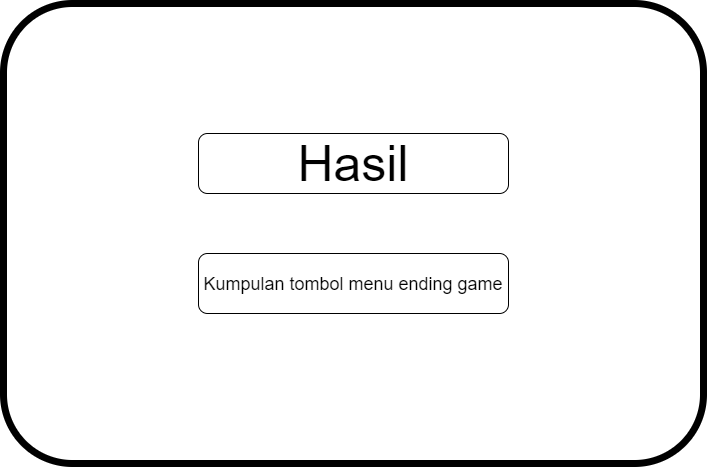
\includegraphics[width=\linewidth-80pt]{pics/low/low4}
		\caption{Tampilan \textit{Low fidelity} halaman setelah menyelesaikan tahap bermain}
	\end{figure}
	

\section{Pembuatan Prototipe}

Pembuatan prototipe dilakukan di atas \textit{platform desktop} dengan menggunakan teknologi yang telah dijelaskan pada spesifikasi sistem. 

	\subsection{Implementasi Halaman \textit{Main Menu}}
	Pada halaman \textit{main menu} terdapat beberapa tombol, yaitu tombol \textit{play}, tombol pengaturan, tombol keluar permainan, tombol kembali, tombol perbesar volume suara, dan tombol perkecil volume suara. Tombol \textit{play}, tombol pengaturan, dan tombol keluar permainan terdapat pada tampilan awal halaman \textit{main menu}. Tombol kembali, tombol perbesar volume suara, dan tombol perkecil volume suara terdapat pada halaman setelah pengguna menekan tombol pengaturan. Gambar 4.21 merupakan tampilan halaman menu utama dan Gambar 4.22 merupakan tampilan halaman menu pengaturan.
	\begin{figure}
		\centering
		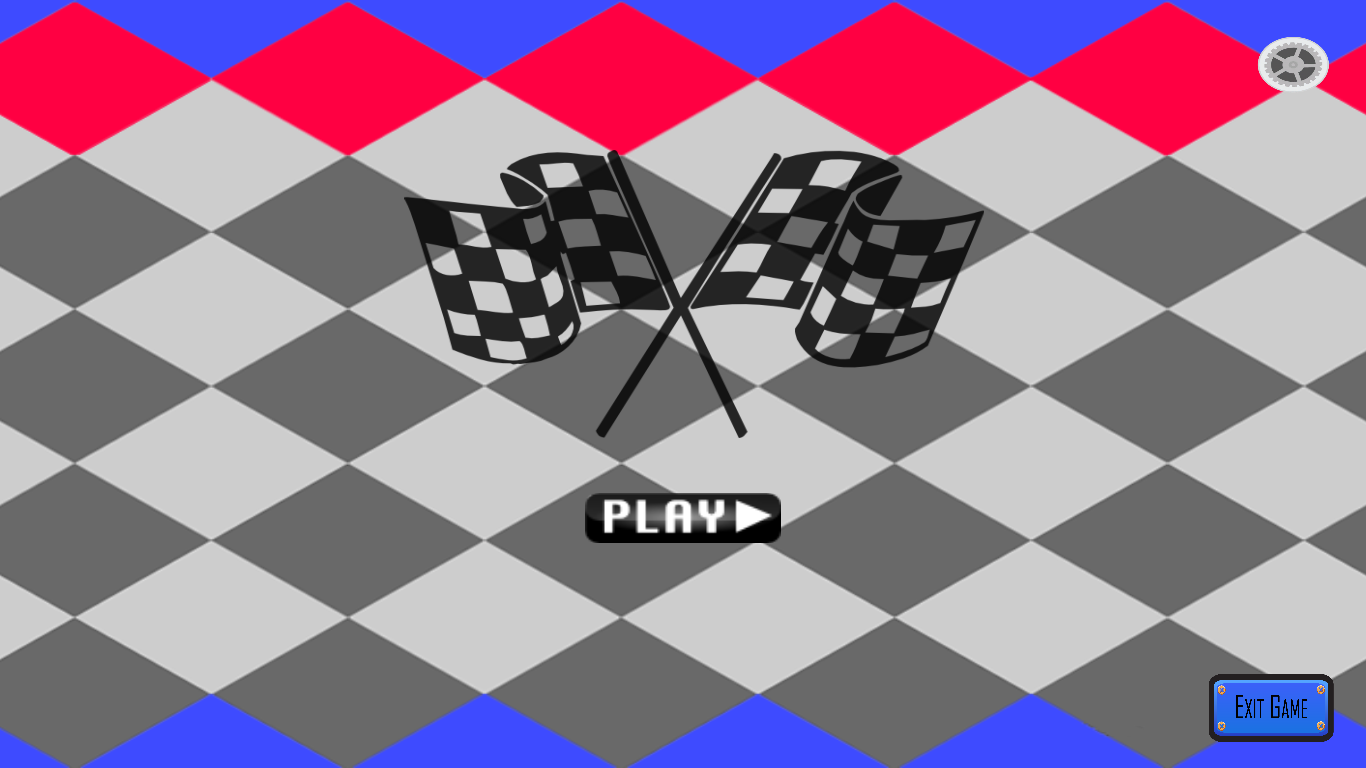
\includegraphics[width=\linewidth-40pt]{pics/prototipe/menu1}
		\caption{Tampilan menu utama}
	\end{figure}
	\begin{figure}
		\centering
		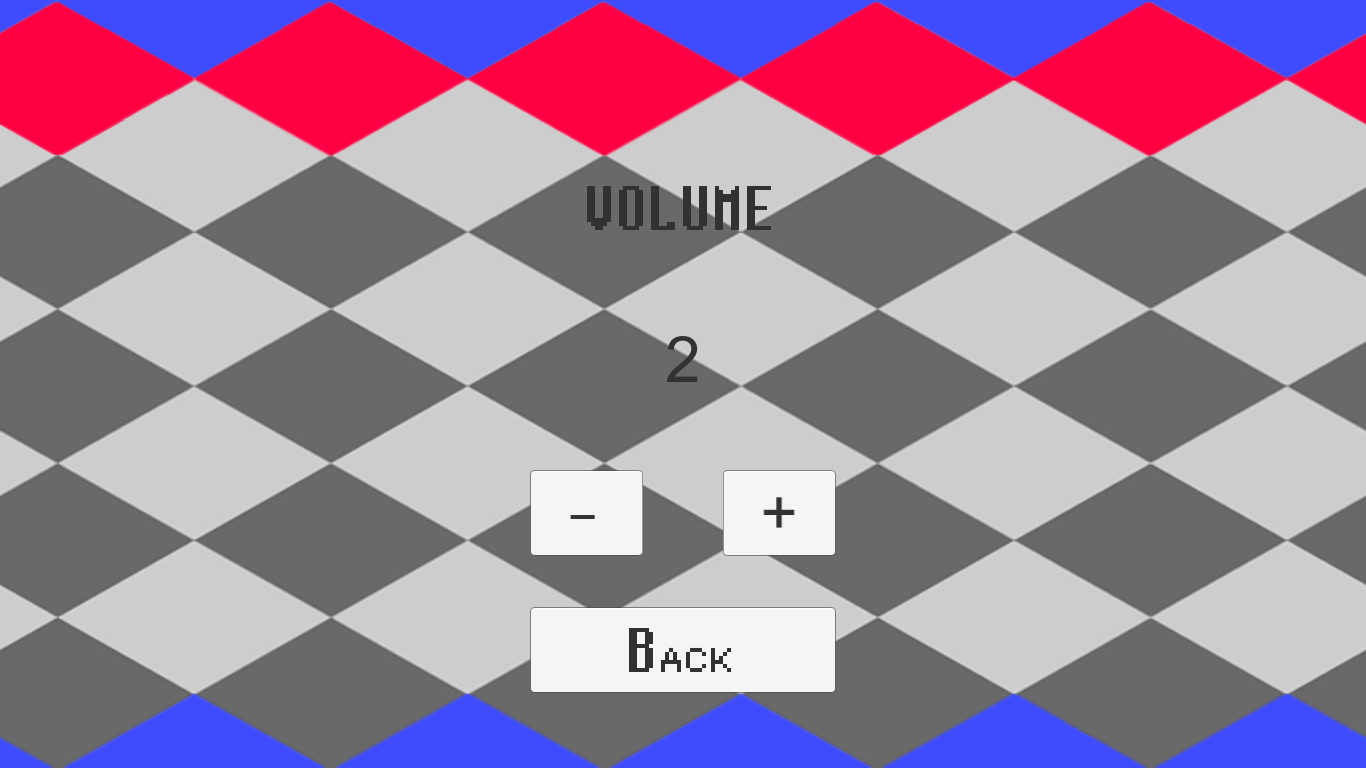
\includegraphics[width=\linewidth-40pt]{pics/prototipe/menu2}
		\caption{Tampilan menu pengaturan}
	\end{figure}
	\subsection{Implementasi Tahap 1}
	Pada tahap pertama dalam permainan, pengguna hanya diminta untuk menekan tombol "\textit{run}" yang berada di bawah sebelah kanan kotak bagian tengah. Tujuan dari tahap ini adalah mengenalkan cara bermain kepada pengguna yaitu dengan menekan tombol hijau di bawah kanan kotak bagian tengah akan menjalankan apa yang ditulis dalam kotak bagian tengah. Gambar 4.23 merupakan tampilan dari tahap pertama.
	\linebreak\linebreak
	Setelah pengguna menyelesaikan ini diharapkan pengguna tau cara menjalankan perintah yang telah ditulis. Setelah menyelesaikan tahap pertama, pengguna akan ditampilkan halaman untuk menentukan apakah ingin melanjutkan ke tahap berikutnya, kembali ke tahap pertama, atau kembali kehalaman \textit{main menu}. Semua perintah tersebut dibuat menggunakan tombol pada bagian bawah penanda berhasil atau tidak pengguna mengerjakan tahap pertama. Terdapat juga penjelasan dari apa yang telah dikerjakan pada tombol rahasia yang ada pada tampilan agar pengguna dapat lebih memahami maksud dari tahap ini. Gambar 4.24 merupakan tampilan berhasil menyelesaikan tahap pertama dan Gambar 4.25 merupakan tambilan gagal menyelesaikan tahap pertama.
	\begin{figure}
		\centering
		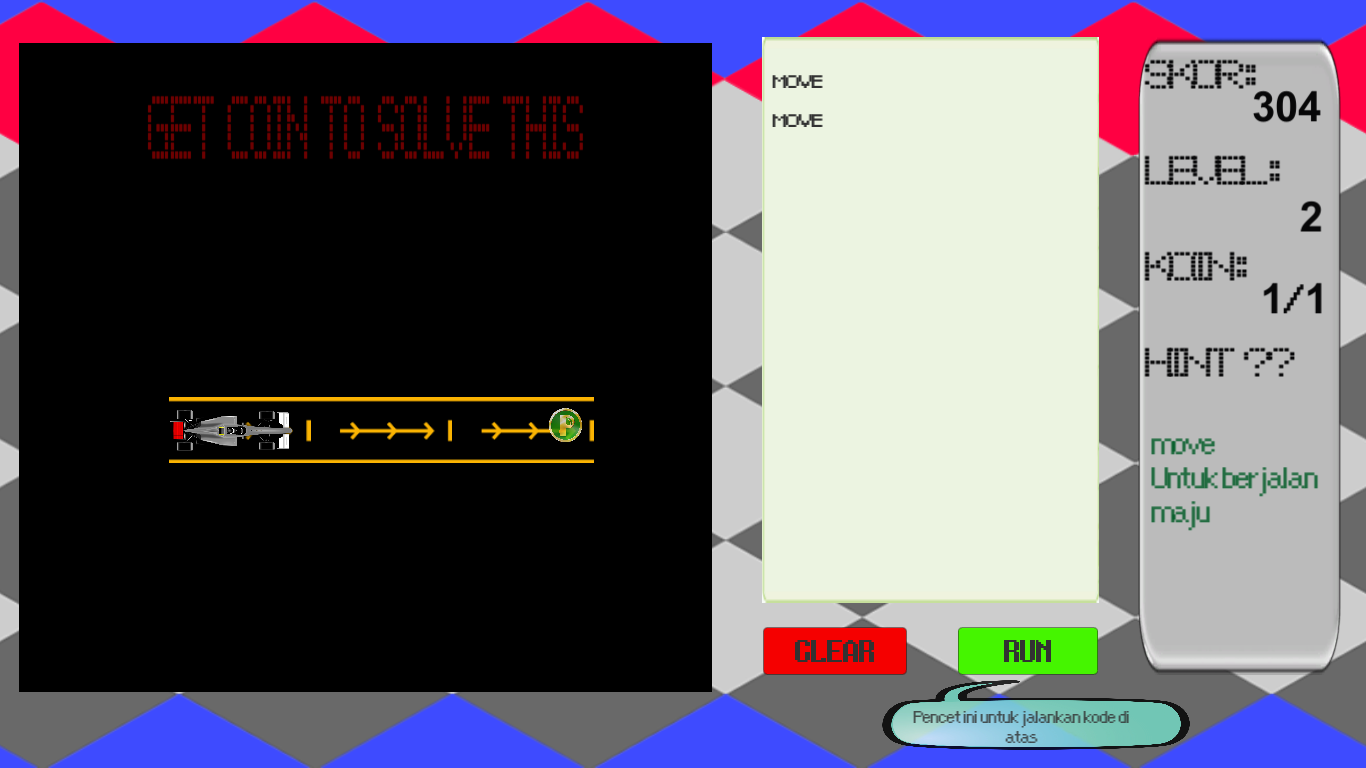
\includegraphics[width=\linewidth-40pt]{pics/prototipe/tahap1}
		\caption{Tampilan tahap 1: Pengenalan cara menjalankan mobil}
	\end{figure}
	\begin{figure}
		\centering
		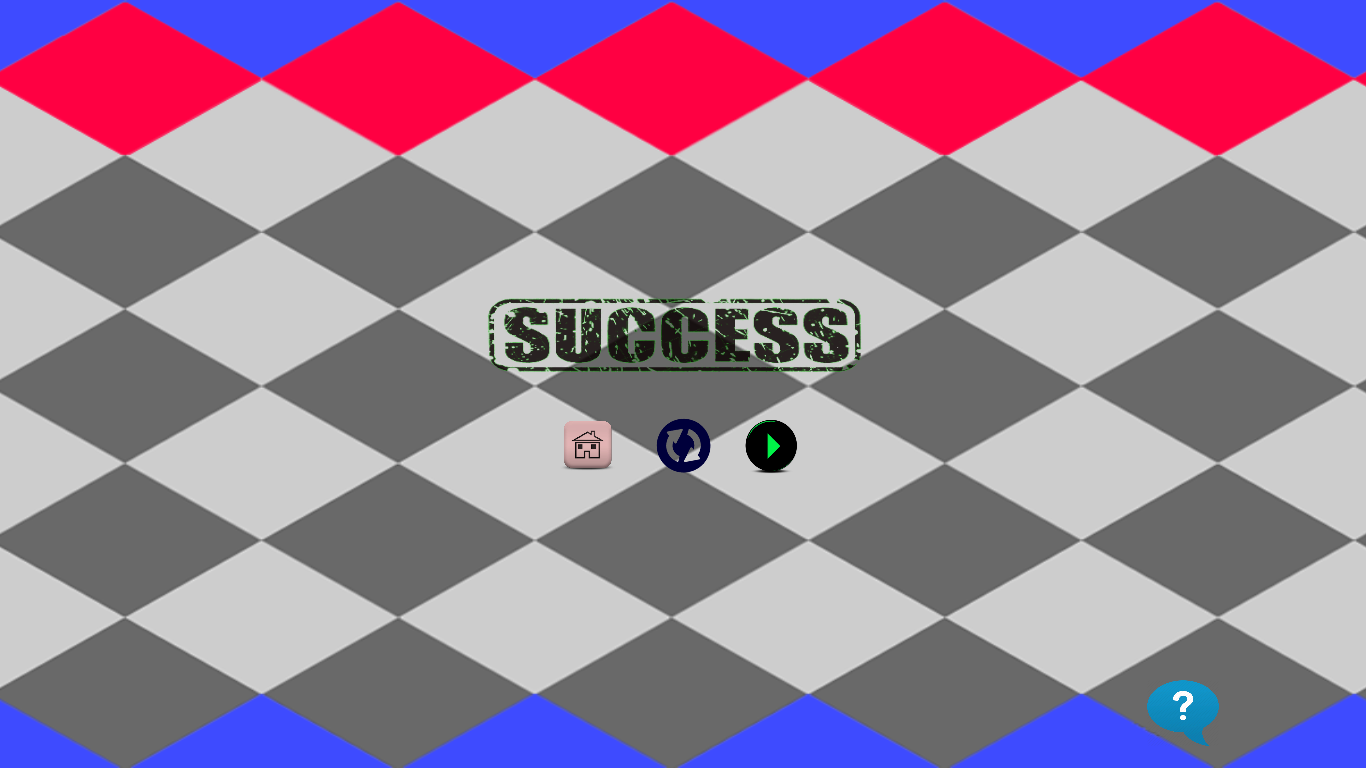
\includegraphics[width=\linewidth-40pt]{pics/prototipe/ending1}
		\caption{Tampilan setelah berhasil menyelesaikan tugas tahap 1}
	\end{figure}
	\begin{figure}
		\centering
		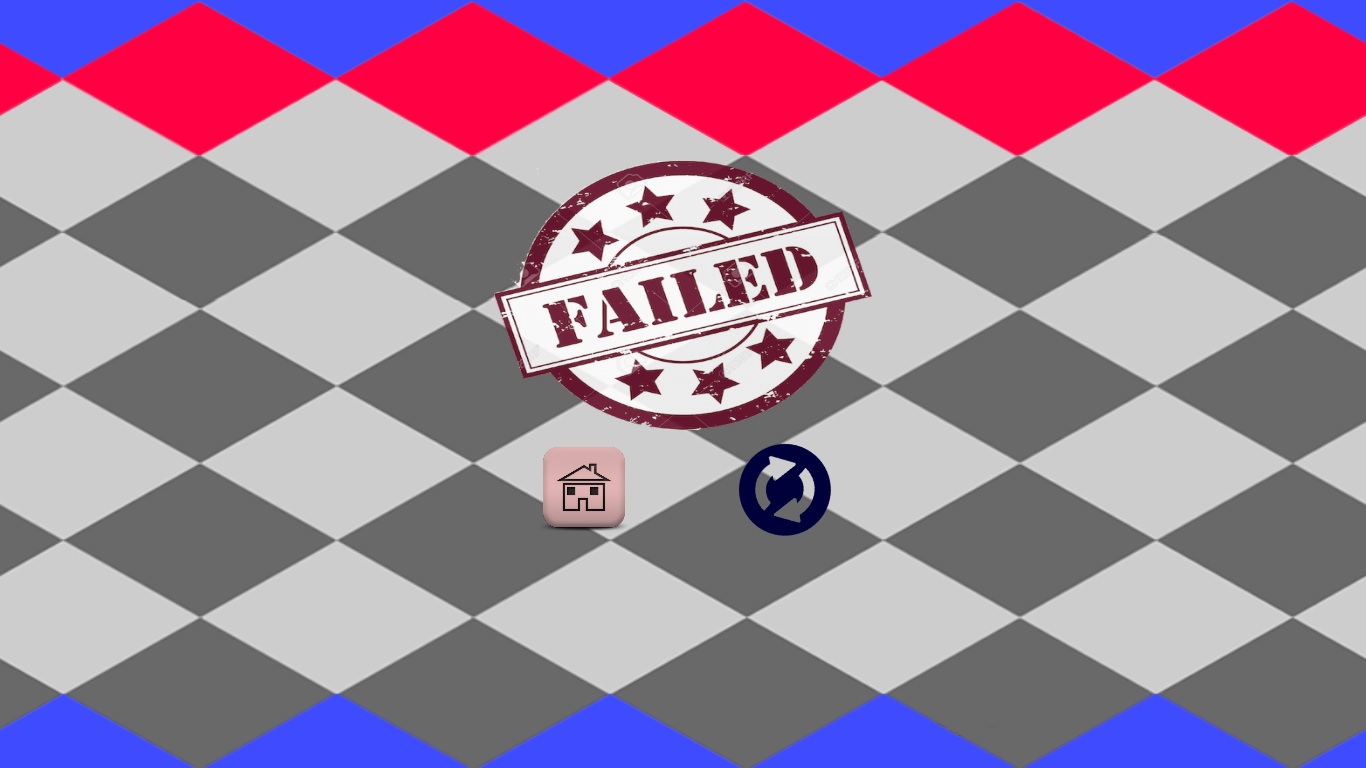
\includegraphics[width=\linewidth-40pt]{pics/prototipe/ending2}
		\caption{Tampilan setelah gagal menyelesaikan tugas tahap 1}
	\end{figure}
	\subsection{Implementasi Tahap 2}
	Pada tahap ini, pengguna hanya diminta untuk menekan tombol "\textit{run}" kembali. Namun pada tahap ini ditampilkan sebuah perintah baru dalam tulisan kode kotak bagian tengah. Perintah yang baru adalah "\textit{turn(L)}" dan sebuah tulisan bantuan baru yang menjelaskan perintah tersebut. Tujuan dari tahap ini adalah mengenalkan perintah baru dan membuat pengguna terbiasa akan menjalankan fitur dari setiap tahap. Untuk bagian setelah selesai tahap maka digunakan hal yang sama pada tahap pertama. Tampilan untuk tahap dua akan terlihat pada Gambar 4.26.
	\begin{figure}
		\centering
		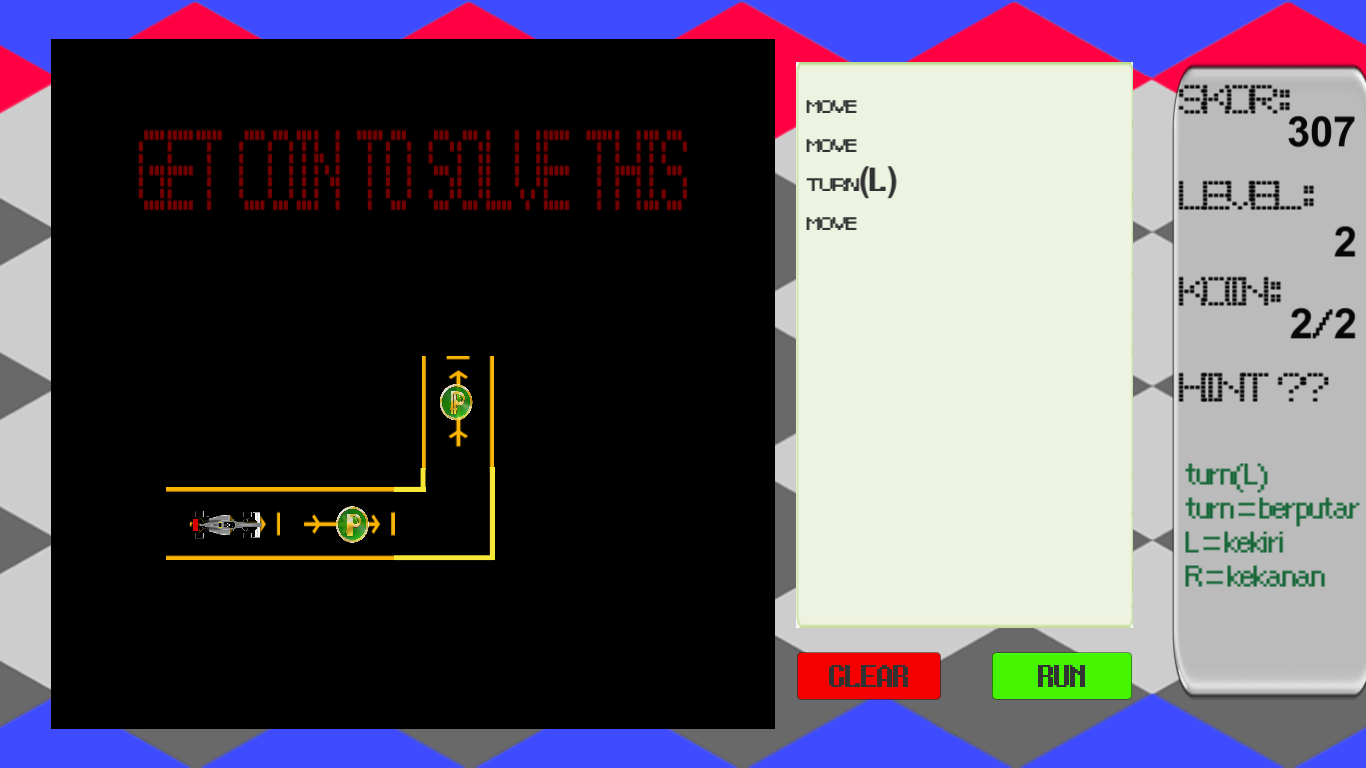
\includegraphics[width=\linewidth-40pt]{pics/prototipe/tahap2}
		\caption{Tampilan tahap 2: Perkenalan perintah "\textit{move}" dan "\textit{turn}"}
	\end{figure}
	\subsection{Implementasi Tahap 3}
	Pada tahap tiga pengguna diminta untuk menyelesaikan masalah yang sedang dihadapi oleh pembalap. Pada tahap ini pengguna diminta untuk menuliskan kode pada kotak bagian tengah. Pada tahap ini user harus menuliskan perintah dari pada yang telah ditampilkan oleh tahap sebelumnya. Tujuan dari tahap ini adalah mengenalkan cara penyelesaian masalah secara utuh, melatih daya ingat hingga melakukan menerapan solusi dari masalah yang telah dipaparkan pada tahap ini. Bagian selesai tahap ini tetap menggunakan tampilan yang sama seperti pada tahap sebelumnya. Tampilan untuk tahap tiga terlihat pada Gambar 4.27.
	\begin{figure}
		\centering
		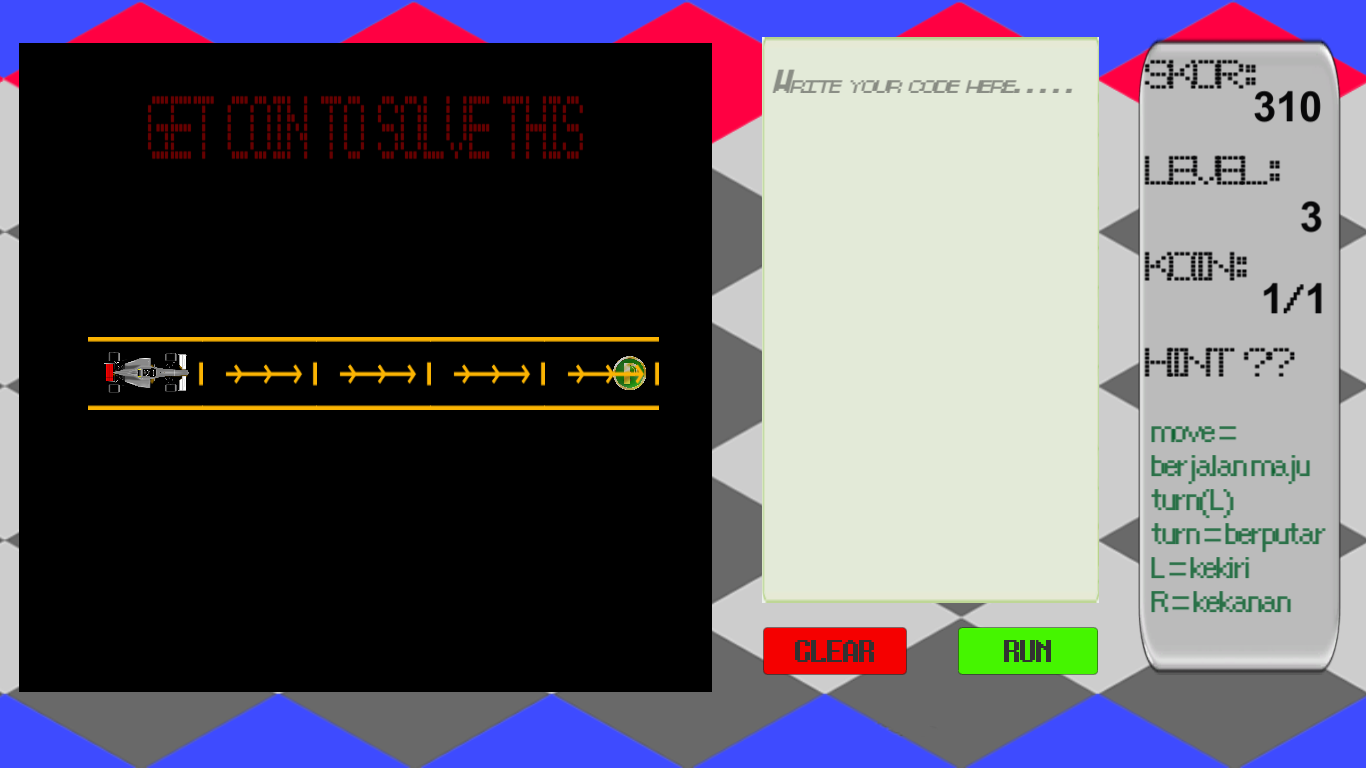
\includegraphics[width=\linewidth-40pt]{pics/prototipe/tahap3}
		\caption{Tampilan tahap 3: Pengenalan menyelesaikan tahap secara keseluruan dengan menggunakan perintah dari dua tahap sebelumnya}
	\end{figure}
	\subsection{Implementasi Tahap 4}
	Pada tahap ini pengguna ditampilkan sebuah perintah baru yaitu "\textit{loop}" sesuai dengan Gambar 4.28. Perintah ini untuk memotong beberapa perintah jika terjadi pengulangan. Pengguna hanya diminta menekan tombol "\textit{run}" saja. Untuk bagian setelah selesai tahap maka digunakan hal yang sama pada tahap pertama.
	\begin{figure}
		\centering
		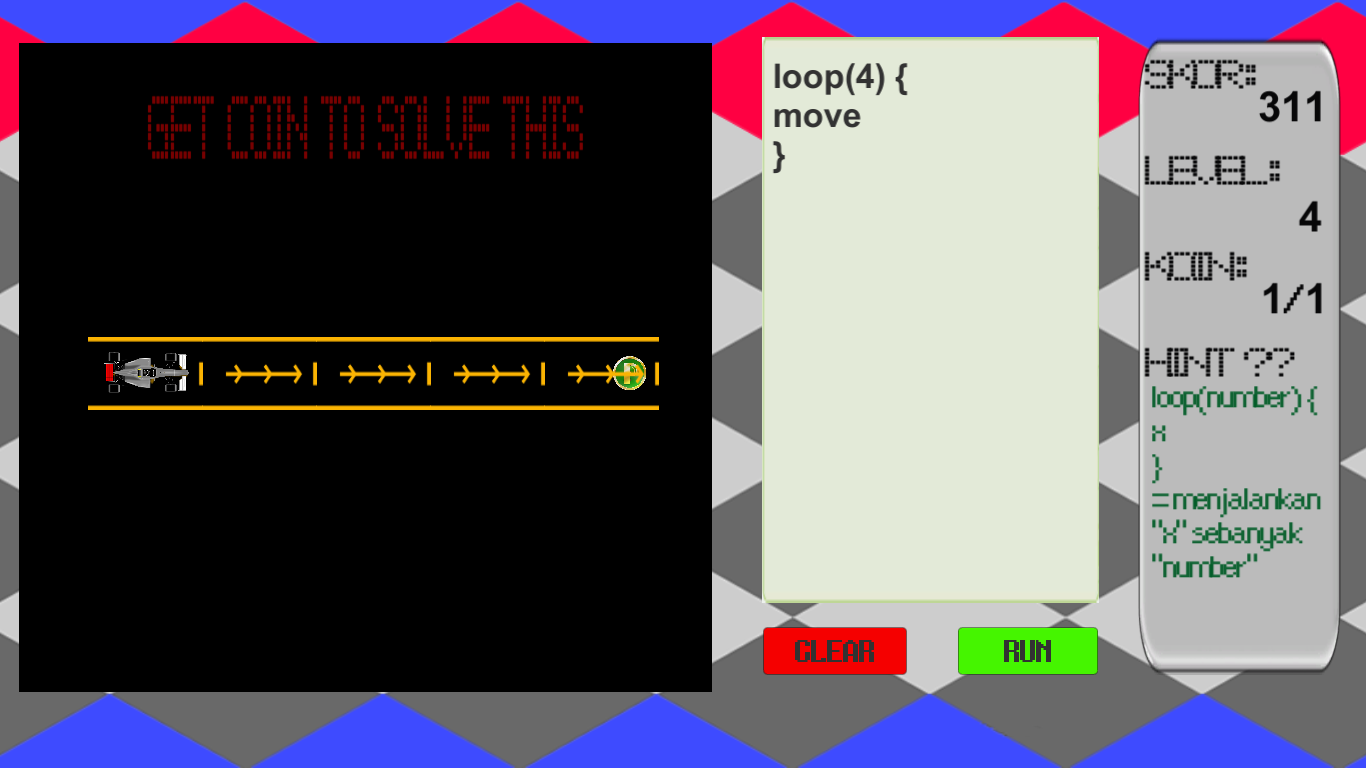
\includegraphics[width=\linewidth-40pt]{pics/prototipe/tahap4}
		\caption{Tampilan tahap 4: Perkenalan perintah "\textit{loop}"}
	\end{figure}
	\subsection{Implementasi Tahap 5}
	Pada tahap ini pengguna diberikan sebuah masalah yang memiliki solusi jika pengguna menggabungkan pengetahuan yang didapat dari beberapa tahap sebelumnya. Untuk bagian setelah selesai tahap maka digunakan hal yang sama pada tahap pertama. Tampilan untuk tahap lima akan terlihat pada Gambar 4.29.
	\begin{figure}
		\centering
		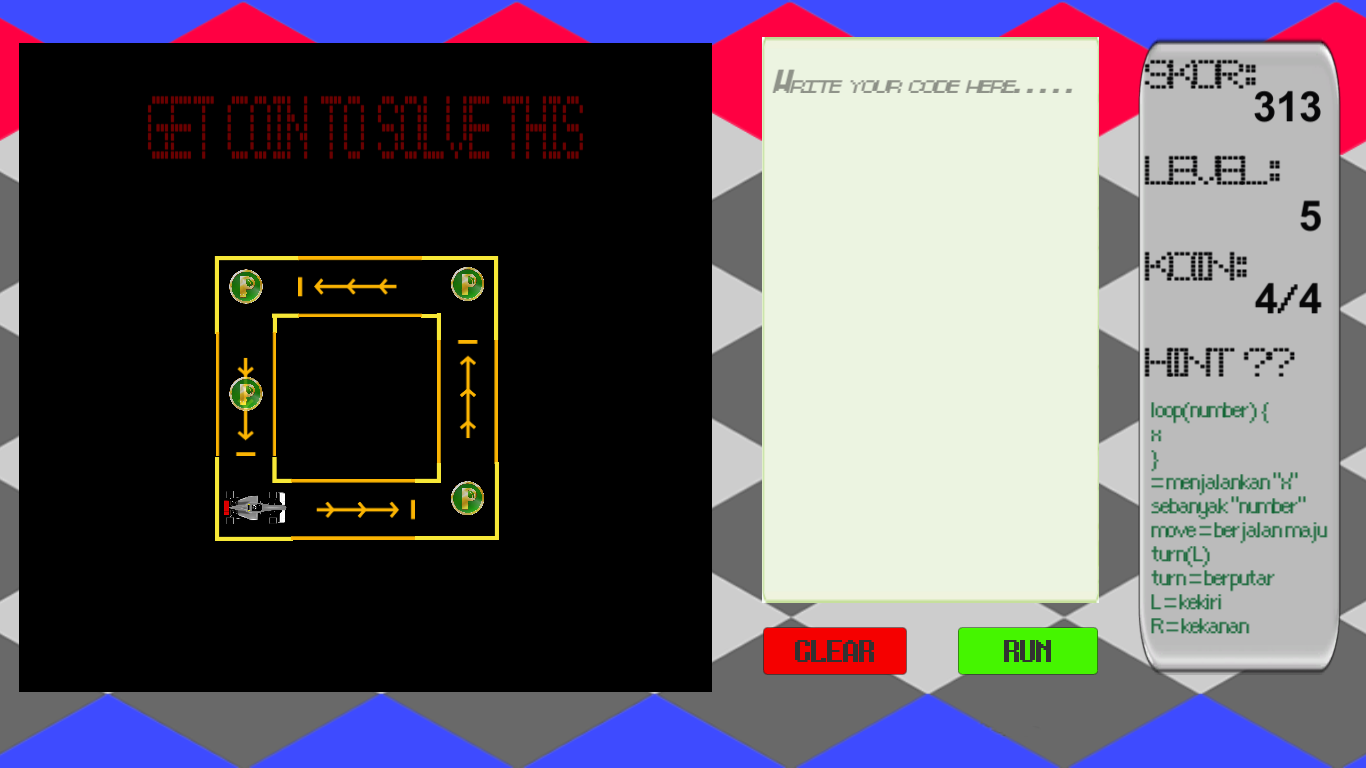
\includegraphics[width=\linewidth-40pt]{pics/prototipe/tahap5}
		\caption{Tampilan tahap 5}
	\end{figure}
	\subsection{Implementasi Tahap 6}
	Pada tahap ini pengguna diberikan sebuah masalah yang paling rumit diantara semua tahap yang ada. Selain pengguna harus mengingat dan menerapkan beberapa pengetahuan dari tahap sebelumnya, pengguna juga harus memikirkan tiap langkah yang diambil. Untuk bagian setelah selesai tahap maka digunakan hal yang sama pada tahap pertama. Gambar 4.30 merupakan tampilan untuk tahap enam ini.
	\begin{figure}
		\centering						
		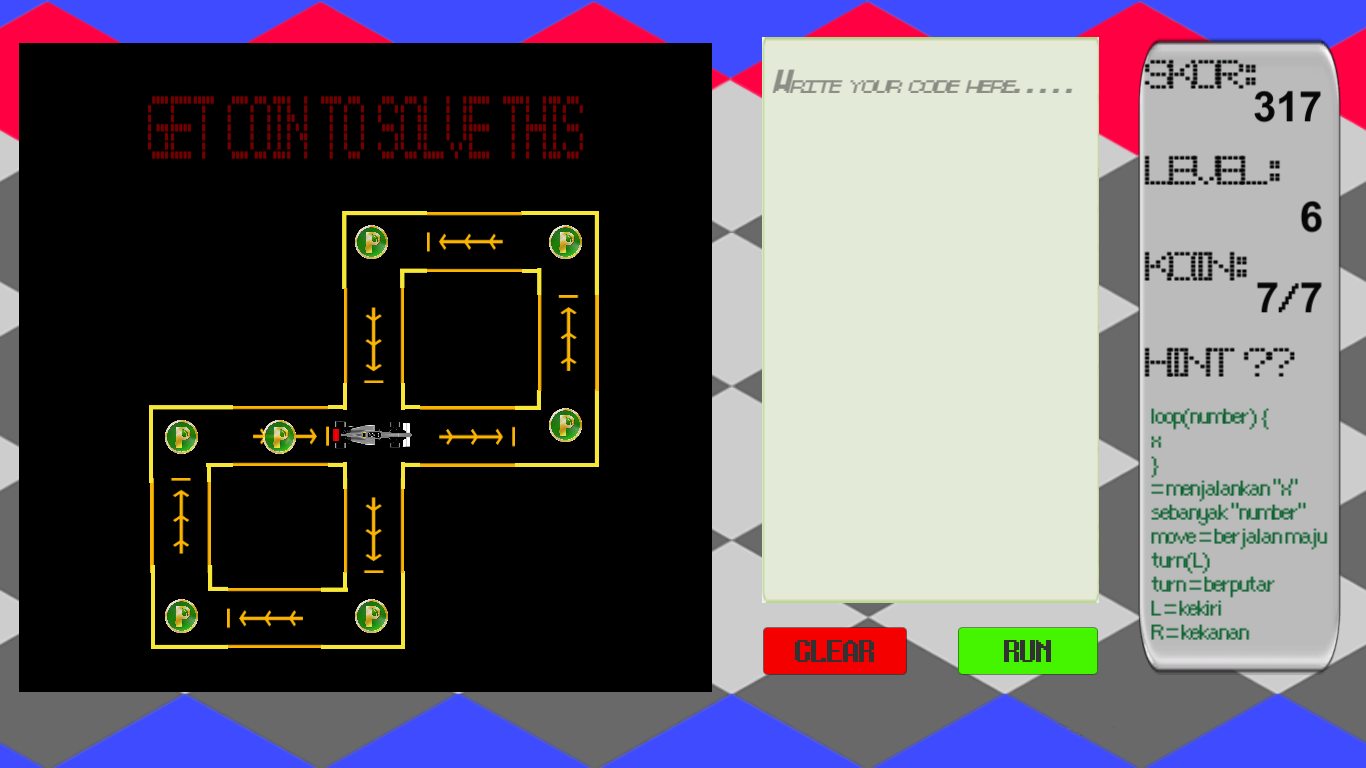
\includegraphics[width=\linewidth-40pt]{pics/prototipe/tahap6}
		\caption{Tampilan tahap 6}
		
	\end{figure}
\section{Pengujian Prototipe dengan \textit{Usability Evaluation}}
Pengujian prototipe dilakukan melalui dua pendekatan, yaitu kualitatif dan kuantitatif. Pendekatan kualitatif dilakukan dengan mengadakan usability testing dengan tujuan agar dapat mengukur efektivitas video permainan dan mendapatkan \textit{design insight}. Sedangkan pengkuran kuantitatif dilakukan melalui kuesioner SUS dengan tujuan untuk mengukur tingkat usability dan kenyamanan menurut pengguna terhadap video permainan.

	\subsection{Perancangan \textit{Usability Testing}}
	Sebelum melakukan UT, terlebih dahulu dibuat skenario. Skenario dibuat berdasarkan pengembangan yang telah disebutkan pada subbab sebelum ini dan apa yang terdapat pada video permainan ini. UT dilakukan secara \textit{task-based} dengan jumlah \textit{task} sebanyak tujuh. Penulis akan memberitahukan tugas apa yang harus dilakukan pengguna, lalu pengguna dibiarkan melakukan sendiri tugas yang diberikan hingga selesai. Setelah selesai, pengguna akan diberikan pertanyaan terkait tugas tersebut. Pertanyaan meliputi perasaan pengguna saat mengerjakan tugas tersebut, apa kesulitan menjalankan tugas tersebut, dan adakah saran pengguna untuk tugas yang telah dilakukannya. Tugas apa saja yang harus dilakukan oleh pengguna akan dirangkum dalam tabel .
	\begin{longtable}{| c | p{4.5cm} | p{7cm} |}
		\caption{Daftar tugas yang digunakan untuk \textit{Usability Testing}} \\
		\hline
		No & Deskripsi Tugas & Keterangan\\ 
		\hline
		\endhead
		1 & Mengeksplorasi halaman menu utama & Pengguna diminta untuk mengeksplorasi semua tombol yang ada pada halaman menu utama\\ 
		\hline
		2 & Menyelesaikan tahap 1 & Pengguna hanya diminta untuk menekan tombol "\textit{run}". Setelah menyelesaikan tahap pertama pengguna diminta untuk mengeksplorasi halaman \textit{reward}. \\ \hline
		3 & Menyelesaikan tahap 2 & Pengguna kembali diminta untuk menekan tombol "\textit{run}" saja karena untuk input perintah sudah tertulis saat tahap ini dimulai. Tujuan dari tahap ini adalah perkenalan perintah yang ada pada permainan. Setelah itu pengguna diminta kembali mengeksplorasi halaman  \textit{reward} \\ \hline
		4 & Menyelesaikan tahap 3 & Pengguna akan mengisi kotak bagian tengah pada permainan dengan perintah yang sudah diperkenalkan sebelumnya. Setelah pengguna yakin dengan perintah yang telah ditulis maka mobil dapat menyelesaikan tahap ini, maka pengguna dapat menjalankan perintahnya. Setelah itu pengguna diminta kembali mengeksplorasi halaman  \textit{reward}\\ \hline
		5 & Menyelesaikan tahap 4 & Pengguna kembali hanya diminta untuk menjalan perintah yang telah ada. Setelah itu pengguna diminta kembali mengeksplorasi halaman  \textit{reward}\\ \hline
		4 & Menyelesaikan tahap 5 & Pengguna akan mengisi kotak bagian tengah dengan perintah namun tingkat kesulitan dinaikkan dari sebelumnya. Setelah itu pengguna diminta kembali mengeksplorasi halaman  \textit{reward}\\ \hline
		5 & Menyelesaikan tahap 6 & Pengguna akan melakukan hal yang sama dengan tahap selanjutnya, namun berbeda masalah yang dihadapi karena harus ada peningkatan kesulitan dalam permainan \\ \hline
	\end{longtable}
	\subsection{Hasil \textit{Usability Evaluation}}
	Pengujian melalui usability evaluation dilakukan terhadap lima belas partisipan dengan karakterisik sesuai dengan persona yang telah dirumuskan sebelumnya. Sebagai rincian, dari delapan responden, diantaranya terdapat tujuh yang termasuk persona 1 dan lima orang termasuk persona 2. Persentase jumlah persona dalam partisipan \textit{usability evaluation} dapat dilihat pada Gambar 4.31.
	\begin{figure}
		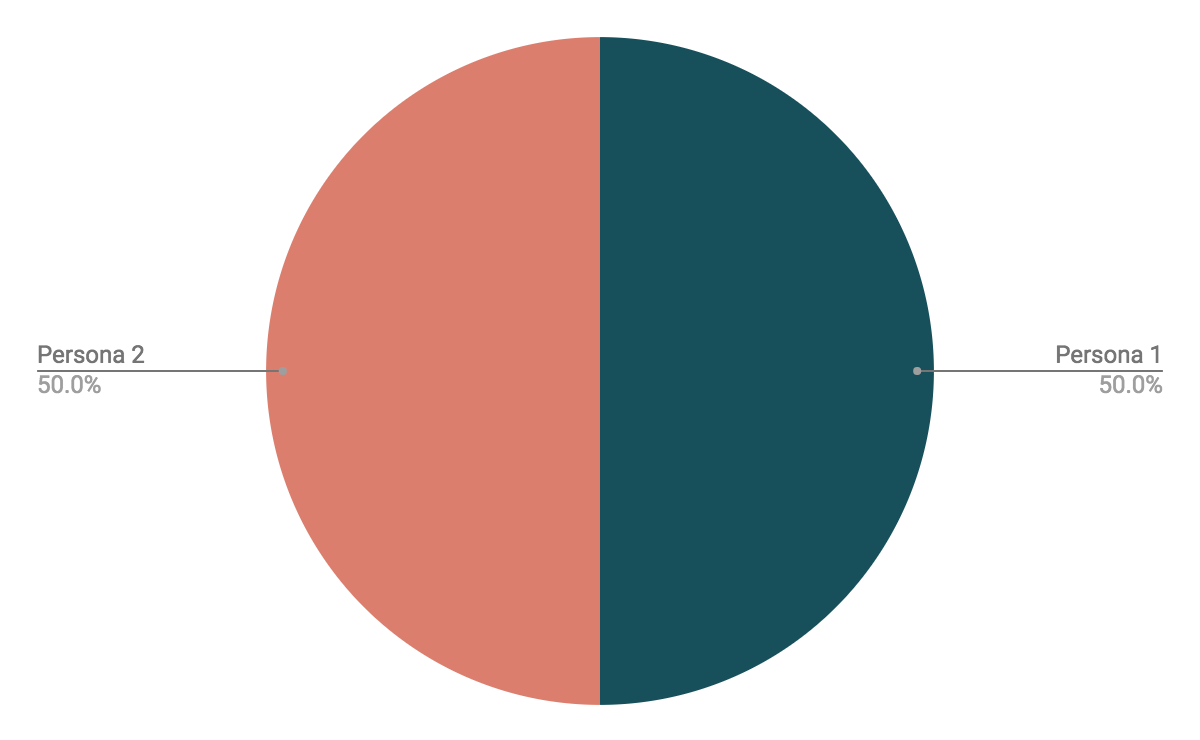
\includegraphics[width=\linewidth]{pics/persentase-jumlah-persona}
		\caption{Persentase jumlah persona partisipan UT}
		\centering
	\end{figure}
	Demografi dari responden \textit{Usability Evaluation} akan dijelaskan pada subbab ini. Sebelas responden berjenis kelamin laki - laki dan empat responden lainnya berjenis kelamin perempuan seperti pada Gambar 4.32.
	\begin{figure}
		%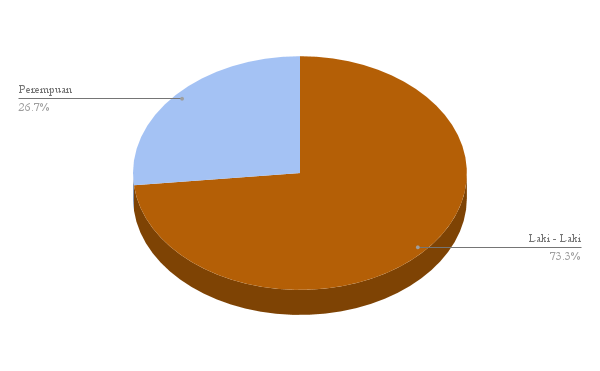
\includegraphics[width=\linewidth]{pics/UT/kelamin}
		\caption{Persebaran responden UT berdasarkan jenis kelamin}
		\centering
	\end{figure}
	Gambar 4.33 merupakan demografi responden berdasarkan umur. Responden yang berumur 22 tahun sejumlah 7 responden (46,7\%), berumur 18 tahun sebanyak 3 responden (20\%), berumur 21 tahun sebanyak 2(13,3\%), dan responden yang berumur 17 dan 19 tahun sebanyak satu responden (6,7\%)
	\begin{figure}
		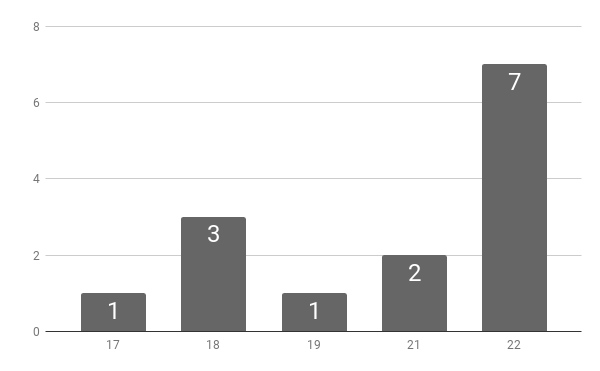
\includegraphics[width=\linewidth]{pics/UT/umur}
		\caption{Persebaran responden UT berdasarkan umur}
		\centering
	\end{figure}
	Responden yang pernah mengambil mata kuliah Dasar Dasar Pemrograman/ Dasar Dasar Pemrograman 1 sebanyak sepuluh orang (66,7\%), dan lima orang (33,3\%) sedang mengambil mata kuliah Dasar Dasar Pemrograman 1 seperti pada Gambar 4.34. Dari sepuluh orang yang pernah mengambil Dasar Dasar Pemrograman tujuh responden (70\%) tidak mengulang dan 3 responden (30\%) mengulang yang digambarkan pada Gambar 4.35.
	\begin{figure}
		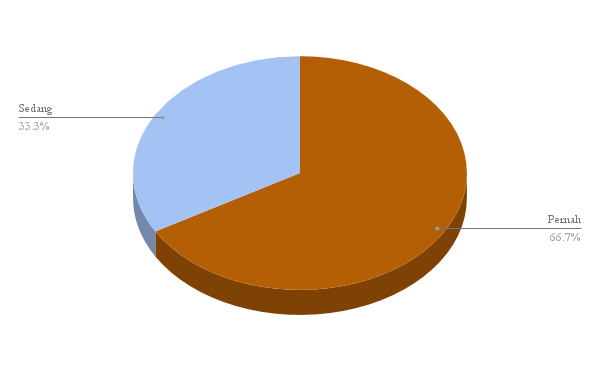
\includegraphics[width=\linewidth]{pics/UT/pernah-sedang}
		\caption{Persebaran responden sedang atau pernah mengambil mata kuliah Dasar Dasar Pemrograman}
		\centering
	\end{figure}
	\begin{figure}
		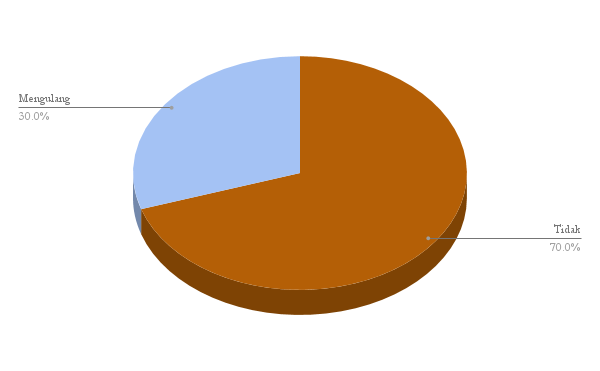
\includegraphics[width=\linewidth]{pics/UT/mengulang}
		\caption{Persebaran mengulang atau tidak bagi yang telah mengambil mata kuliah Dasar Dasar Pemrograman}
		\centering
	\end{figure}
	Seperti yang terdapat pada Gambar 4.36, jenis \textit{game} yang disukai oleh responden bervariasi, 6 orang (\%) menyukai permainan strategi, 3 orang menyukai permainan kartu dan \textit{role-playing game}, dan 1 orang menyukai \textit{clicker, board game}, dan MOBA.
	\begin{figure}
		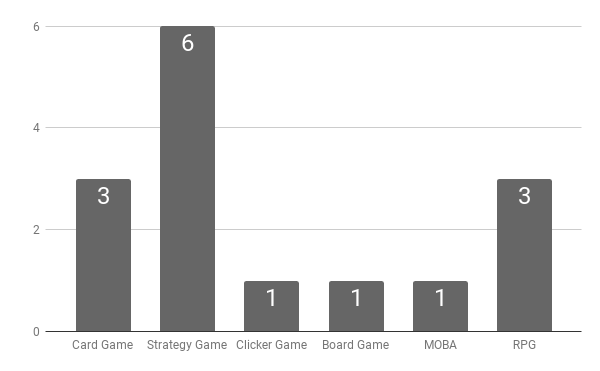
\includegraphics[width=\linewidth]{pics/UT/jenis-game}
		\caption{Persebaran responden UT berdasarkan jenis permainan}
		\centering
	\end{figure}
	\subsubsection{\textit{Usability Testing}}
	Hasil UT terdapat pada Lampiran 3 menunjukkan bahwa partisipan tertarik menggunakan video permainan ini sebagai media pembelajaran pemrograman. Alasan yang dapat disimpulkan dari jawaban partisipan adalah merasa diberikan contoh langsung dalam mengerjakan penyelesaian masalah pemrograman, tampilan yang \textit{to the point}, memberikan efek tantangan yang membuat pengguna sangat ingin mencoba menyelesaikan masalah yang dihadapkan dan desain yang interaktif dan menarik secara visual. Partisipan memberikan saran yang akan digunakan sebagai \textit{design insight} untuk pembuatan prototipe selanjutnya.
	\linebreak\linebreak
	Menurut Sauro (dalam Mifsud, \citeyear{article.sauroMifsud}), efektivitas suatu produk dapat diukur melalui UT, dengan cara menandai partisipan yang berhasil melakukan \textit{task} dengan nilai \textit{binary} "1" dan "0" untuk setiap partisipan yang gagal melakukan \textit{task}, kemudian hasilnya dijumlahkan dan dihitung menggunakan rumus efektivitas yaitu ((jumlah tugas yang selesai / total tugas yang harus diselesaikan) * 100\%).
	\begin{figure}
		\centering
		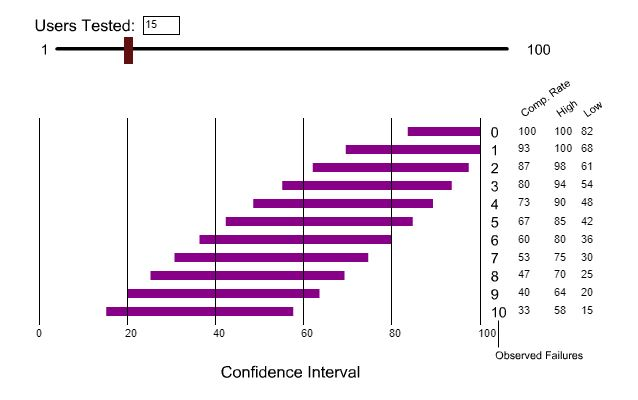
\includegraphics[width=\linewidth]{pics/perhitungan-sauro}
		\caption{Perhitungan efektivitas dalam responden 15 orang (Sauro \citeyear{article.sauroWhat})}
	\end{figure}
	\begin{figure}
		\centering
		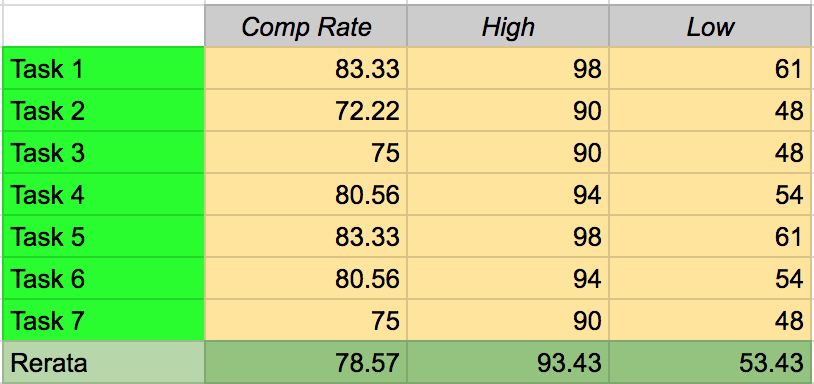
\includegraphics[width=\linewidth]{pics/hasil_sauro}
		\caption{Hasil UT menggunakan perhitungan efektivitas}
	\end{figure}
	\begin{figure}
		\centering
		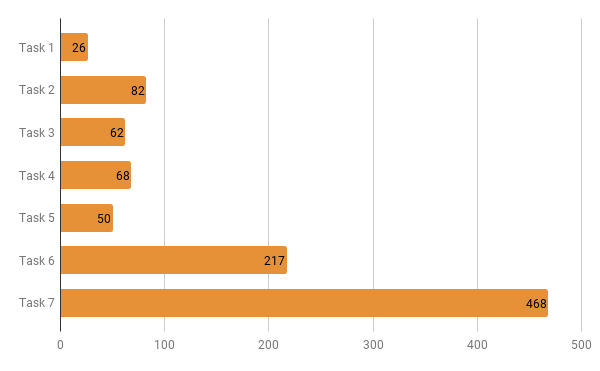
\includegraphics[width=\linewidth]{pics/waktu-UT}
		\caption{Persebaran waktu pengerjaan UT}
	\end{figure}
	Dengan memberikan enam skenario yang dikerjakan oleh responden maka didapati hasil seperti Gambar 4.37. Pada skenario pertama sebesar 83,3\% \textit{task} yang berhasil dikerjakan oleh responden. Skenario kedua dan kelima sebesar 72,2\%, skenario ketiga sebesar 75\%, dan skenario keempat dan keenam sebesar 80,5\%. Dengan menggunakan perhitungan efektivitas maka rerata yang didapatkan adalah 78,57\% dengan batas atas 93,43\% (sangat baik) dan batas bawah 53,42\% (buruk).
	\begin{figure}
		\centering
		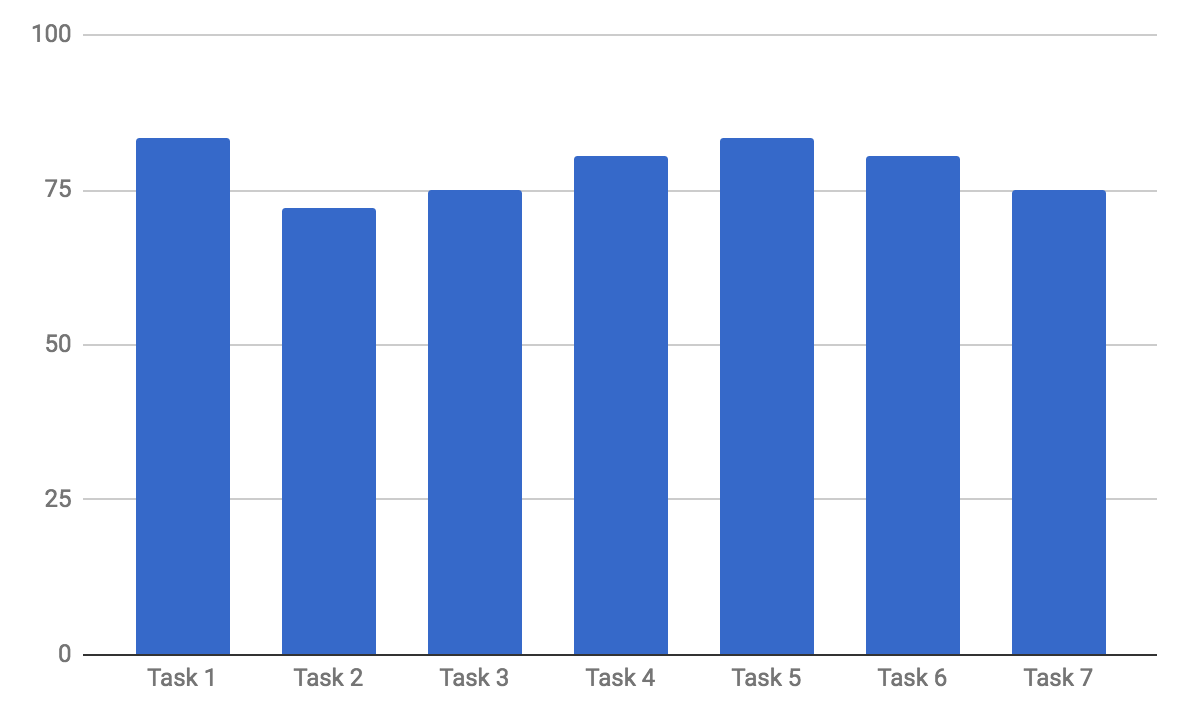
\includegraphics[width=\linewidth]{pics/persebaran-hasil-ut}
		\caption{Persebaran hasil perhitungan UT}
	\end{figure}
	
	Setelah melakukan UT, responden diminta untuk memberikan pendapat tentang sistem ini dan tentunya dikaitkan hubungannya dengan mata kuliah Dasar Dasar Pemrograman 1 atau Dasar Dasar Pemrograman. Berikut pendapat responden terkait sistem ini:
	\begin{itemize}
		\item Lebih menarik karena melihat secara langsung implemantasi dari program yang dituliskan.
		\item Tidak terbatas akan pengetahuan \textit{syntax}, karena lebih ditonjolkan pemahaman konsep.
		\item Memberikan rasa ingin tahu lebih dalam dan sifat \textit{addictive} yang baik karena tiap tahap menarik dengan tingkat kesulitan yang berbeda.
		\item Memberikan cara mengisi waktu luang \textit{gamers} dengan lebih bermanfaat
	\end{itemize}
	\subsection{Rekomendasi}
	Saat melakukan UT, responden memberikan saran sebagai \textit{design insight} untuk memperbaiki sistem yang telah dibuat. \textit{Design insight} yang didapat akan berguna untuk penelitian selanjutnya atau pengembangan selanjutnya dari prototipe ini. Rekomendasi dari responden sebagai berikut:
	\begin{enumerate}
		\item Pengaturan yang ada dalam permainan ini sebaiknya tambah lagi. Penambahan bisa berupa resolusi layar, tentang penulis, cara bermain, dan lain-lain.
		\item Berikan \textit{pop-up} untuk meyakinkan pengguna apakah ingin keluar dari permainan.
		\item Pada bagian \textit{text editor} sebaiknya diberikan nomor baris, \textit{scroll bar}.
		\item Pada saat ingin memulai permainan, sebaiknya diberikan pilihan tahap yang mau dimainkan.
		\item Pada saat mulai melakukan penulisan kode, sebaiknya diberikan indikator apakah terdapat penulisan yang salah dalam kode dengan merubah warna tombol tertentu.
		\item Berikan hasil evaluasi apakah itu yang terbaik atau bukan meskipun sama sama berhasil.
		\item Gunakan aset yang lebih manarik.
		\item Jumlah \textit{level} diperbanyak.
		\item Berikan detail konsep yang ada dalam materi ajar berupa text pada suatu titik didalam permainan.	
	\end{enumerate}
	